\documentclass[parskip]{scrreprt}

%%%%%%%%%%%%%%%%%%% Pakete %%%%%%%%%%%%%%%%%%%%%%%%%%%%%%%%%%%%%%%%%%%%%%%%

%%% Sprache und Eingabecodierung %%%
\usepackage[greek, ngerman, main=english]{babel}		
% Sprachpaket greek damit griechische Buchstaben (z.B. im Literaturverzeichnis) keine Probleme machen mit main= die standardsprache für das Dokument festlegen, damit werden automatische Überschriften wie Inhaltsverzeichnis/Table of Contents in der richtigen Sprache gesetzt

\usepackage[utf8]{inputenc}							% codierung damit man Umlaute direkt schreiben kann
\usepackage[T1]{fontenc}							% auch was mit codierung zu tun

%%% Schriftart und Form %%%
\usepackage{lmodern}								% Schriftart LatinModern Vektorisiert für schöneres PDF
\usepackage[onehalfspacing]{setspace}				% Korrekter Zeilenabstand nach IPMB Vorgabe
\usepackage[left=2.50cm, right=2.50cm, top=2.50cm, bottom=2.50cm]{geometry}	% Seitenränder nach Vorgabe von IPMB
\usepackage[autooneside=true, headsepline]{scrlayer-scrpage} % schönere Kopfzeile

%%% Chemie, Biologie, Mathematik %%%
\usepackage{dnaseq}									% Für einzelne Sequenzen
\usepackage{texshade}								% Für alignierte Sequenzen 
%%%%%%%%%%%%%%%%%% !!! ACHTUNG !!! dnaseq vor texshade vor mhchem vor graphicx einbinden !!! ACHTUNG !!! %%%%%%%%%%%%%%%%%%

\usepackage[version=4]{mhchem}						% Chemische Formeln
\usepackage{siunitx}								% SI Einheiten
\usepackage{amsmath}								% für schönere Formeln
\usepackage{listings}

%%% Tabellen und Abbildungen %%%
\usepackage{array}
\usepackage{tabulary}
\usepackage{tabularray}
\usepackage{tabularx}
\usepackage{adjustbox}
\usepackage{longtable}								% Tabelle mit Seitenumbrüchen
\usepackage{booktabs} 								% für schöne Linien in Tabellen
\usepackage{multirow}								% Mehrere Reihen in einer Tabelle zusammenfassen
\usepackage{rotating}								% für Tabellen im Querformat
\usepackage{subfigure}								% für mehrere Unterabbildungen in einer Abbildung
\usepackage{graphicx}								% für Größenänderungen für Grafiken
\graphicspath{ {./figures/} }
%\usepackage{float}									% um floats (z.B. Bilder) an Ort und Stelle zu fixieren mit [H]


\usepackage{caption}
\usepackage{threeparttable}
\usepackage[labelfont=bf,font={footnotesize}]{caption}


\usepackage{acronym}								% Abkürzungen
\usepackage{bib/cell}									% Zitierstil Cell


\usepackage{lipsum}									% Blindtext zum Testen

\usepackage[hidelinks]{hyperref}					
\hypersetup{
    colorlinks=true,
    linkcolor=black,
    filecolor=magenta,      
    urlcolor=blue,
    pdftitle={Overleaf Example},
    pdfpagemode=FullScreen,
	citecolor=black,
    }

\urlstyle{same}
% Hyperlinks [hidelinks] um linkboxen zu deaktivieren (möglichst zum Schluss einbinden, da es sich anderen Paketen anpasst)

%%%%%%%%%%%%%%%%%%% KOMA-Script Einstellungen %%%%%%%%%%%%%%%%%%%%%%%%%%%%%
\usepackage{scrhack}								% Anpassung von anderen Paketen an KOMA-Script zur besseren Kompatibilität. Zuletzt Einbinden!

\emergencystretch=50pt								% Vergrößert Wortzwischenraum notfalls, wenn sonst die Zeile überläuft

\clubpenalty = 10000								% Verhindern von Schusterjungen
\widowpenalty = 10000								% Hurenkindern
\displaywidowpenalty = 10000						% und vor Formeln

% Einstellen der Kopfzeile
\clearscrheadfoot									% Ohne Voreinstellungen beginnen
\automark{chapter}									% automatisches Aktualisieren von sections
\ihead{\headmark}									% innerer Kopf: aktuelle section
\ohead{\pagemark}									% äußerer Kopf: Seitenzahl



%%%%%%%%%%%%%%%%%%% Schriftart für Überschriften einstellen %%%%%%%%%%%%%%%
\setkomafont{title}{\sffamily}						% Festsetzen der Überschriftart auf Sans Serif
\setkomafont{disposition}{\usekomafont{title}}		% Festsetzen der weiteren Unterüberschriften auf Sans Serif
\setkomafont{author}{\usekomafont{title}}
\setkomafont{date}{\usekomafont{title}}
\setkomafont{caption}{\sffamily\small}					% Festsetzen der Captions auf Sans Serif klein
\setkomafont{captionlabel}{\usekomafont{caption}\bfseries\small}	% Festsetzen der Captionlabels auf Sans Serif Fett klein

%%%%%%%%%%%%%%%%%%% Definitionen für Titelseite %%%%%%%%%%%%%%%%%%%%%%%%%%%
\newcommand{\workauthor}{Ian Dirk Fichtner}
\newcommand{\worktitle}{ Applying NCEM and MISTy on MIBI-TOF colorrectal cancer data as a primer for spatial cell-cell communication benchmarking}
\newcommand{\studentid}{3404046}
\newcommand{\birthplace}{Santa Fé de Bogotá, Colombia}
\newcommand{\workplace}{Heidelberg}
\newcommand{\workstart}{07.~November~2022}
\newcommand{\workstop}{15.~February~2023}
\newcommand{\submissiondate}{\today}
\newcommand{\institute}{German Cancer Research Center}
\newcommand{\department}{Computational Genomics and Systems Genetics}
\newcommand{\supervisor}{Elyas Heidari}
\newcommand{\headrg}{Prof. Dr. Oliver Stegle}
\newcommand{\worktype}{Internship report}

%%%%%%%%%%%%%%%%%%% Paketeinstellungen %%%%%%%%%%%%%%%%%%%%%%%%%%%%%%%%%%%%%

\lstset{							% Einstellungen für listings
	frame=tb,						% Horizontale Linien oben und unten
	numbers=left,					% Zeilennummern auf der linken Seite
	basicstyle=\ttfamily\small,		% Schrift Monospace klein
%	language=,						% Festlegen der Programmiersprache
	tabsize=2,						% Tabs sind 2 Leerzeichen breit
}

\sisetup{
	per-mode=fraction,				% macht Brüche bei Einheiten
	output-decimal-marker={,},		% gibt "," als Dezimaltrennzeichen aus
	separate-uncertainty,			% Unsicherheit mit +-
	table-align-uncertainty = true,	% Ausrichtung am +- in Tabellen
}

\begin{document}

%%%%%%%%%%%%%%%%%%% Titlepage für Bachelor/Masterarbeit %%%%%%%%%%%%%%%%%%%
\begin{titlepage}
	\centering
	{\Large Ruprecht-Karls-Universität Heidelberg\\
			Fakultät für Biowissenschaften\\
			Bachelorstudiengang Molekulare Biotechnologie\\}
	
	{\usekomafont{title}
		{\vspace{\stretch{2}}\Huge \worktitle{}}}
	
	\vspace{\stretch{2}}
	{\Large \worktype{}}
	
	\vspace{\stretch{2}}
	
	{\large
	\begin{tabular}{r l}
		Autor &\workauthor{}\\
		Supervisor &\supervisor{}\\
		Institute &\institute{}\\
		Department &\department{}\\
		Head of research group &\headrg{}\\
	\end{tabular}
	}
	\vspace{1cm}

	\workstart \quad- \workstop
	\vspace{1cm}
	
	------------------------------------------------------

	\submissiondate, Heidelberg (Signature)
		
	\vspace{\stretch{2}}
	
	
	
\end{titlepage}
%%%%%%%%%%%%%%%%%%% /Titlepage für Bachelor/Masterarbeit %%%%%%%%%%%%%%%%%%

\thispagestyle{plain}
The present \worktype{} was carried out at the \institute{} in \workplace in time between \workstart{} and \workstop{}.

\begin{center}
	\begin{tabular}{rl}
		First Referee: &\headrg\\
		&\department\\
		&\institute\\
		Supervisor: &\supervisor\\
		&\\ % Nur für Master
%		Zweitgutachter der Arbeit &Dr. Matthias Schlesner\\
%		&Computational Oncology\\
%		&eilslabs, Deutsches Krebsforschungszentrum\\
	\end{tabular}
\end{center}










\vspace{\stretch{4}}
I herewith declare that:
\begin{enumerate}
	\item I wrote this \worktype independently under supervision and that I did not used other sources and supporting materials than those indicated;die Übernahme wörtlicher Zitate aus der Literatur und dem Internet sowie die Verwendung der Gedanken anderer Autoren an den entsprechenden Stellen innerhalb der Arbeit gekennzeichnet wurde
	\item the adoption of quotation from the literature/internet as well as thoughts from other authors are indicated in the thesis;die Übernahme wörtlicher Zitate aus der Literatur und dem Internet sowie die Verwendung der Gedanken anderer Autoren an den entsprechenden Stellen innerhalb der Arbeit gekennzeichnet wurde
	\item I have not submitted this \worktype for any other examination
\end{enumerate}

I am aware of the fact that a false declaration will have legal consequences.

% 3,5cm Abstand nach oben
\vspace{\stretch{1}}
% Ort, Datum
\workplace{}, der \submissiondate{}
\vspace{1,5cm}
% 8 cm breite Linie für die Unterschrift
\begin{center}
	\begin{minipage}[t]{8cm}
		% gepunktete Linie
		\centering \dotfill \\
		% Text unter der Linie
		\workauthor{}
	\end{minipage}
\end{center}


\vspace{\stretch{1}}
\tableofcontents
\chapter*{Abstract}
\addcontentsline{toc}{chapter}{Abstract}


Prior to the emergence of spatial-omics technologies, cell-cell communication (CCC) methods relied on prior knowledge about interacting features between cells. The measure of correlation between putative ligand-receptor interactions are a common approach to this end. Novel spatially-resolved omics technologies like MIBI-TOF and MERFISH enable the measurement and characterization of feature patterns in space. Novel CCC methods followed which attempt to leverage the spatial dimension. These methods face four main challenges: (1) lack of a consensus on how to define and approach CCC, (2) vast diversity of spatial-omics technologies with different output types and properties, (3) high level of artifacts and uncertainty in upstream steps and (4) lack of ground truth for validation.

In the present study, the aim was to set the groundwork towards benchmarking spatially-resolved CCC methods by applying recent spatial CCC methods NCEM and MISTy to a colorectal tumour dataset. We analyzed their potential weaknesses and attempted to reach a comparable output.

The linear NCEM model was applied to the dataset and the interaction term tensor was summarised via two different transformations to achieve a cell-type level sender-receiver effect matrix. Furthermore, erroneous cell-type annotation due to upstream effects was simulated via shuffling the annotations of varying fractions of randomly selected cells. The results showed a high sensitivity towards cell-type annotation as shuffling 10% of the cells' cell-types reached similar explained variance ($R^2$) values to 100% annotation randomization.

MISTy was applied by defining the "intra-view" and a "para-view". As opposed to NCEM, MISTy doesn't model batch and conditions directly; it is run on an individual sample basis and the results are summarized via the mean and standard deviation. When examining the improvement of explained variance ($R^2$) attributed to the "para-view", high standard deviation for all features was observed. This shows the necessity of better sample integration or the assessment of experimental conditions for intermediate step interpretability.

MISTy was customized to yield a similar output to NCEM. However, predictor-target importances were only obtained on the individual sample level.


\pagenumbering{roman}
\setcounter{page}{1}



%\listoffigures
%\addcontentsline{toc}{chapter}{List of Figures}
%\listoftables
%\addcontentsline{toc}{chapter}{List of Tables}


{\setlength{\parskip}{0.2cm}
%	Abkürzungsverzeichnis
\chapter*{Abbreviations}
	\begin{acronym}[ABCDEFGHIJK]
		% A B C D E F G H I J K L M N O P Q R S T U V W X Y Z		
		% Abkürzungen
		%\acro{acronym}{full name}
		
		% Formelzeichen
		%\acro{acronym}[$ Formelzeichen $]{full name}
		
		% als benutzt markierte Acronyme	
		%\acused{acronym}
		
	\end{acronym}
}

\begin{table}[!ht]
    \raggedright
    \begin{tabular}{ll}
        \textbf{CCC} & Cell-cell communication \\ 
        \textbf{CCI} & Cell-cell interactions \\ 
        \textbf{CVAE} & Conditional variational autoencoder \\ 
        \textbf{Ecad} & E-cadherin \\ 
        \textbf{FISH} & Fluorescence in-situ hybridization \\ 
        \textbf{FRET} & Fluorescence resonance energy rransfer \\ 
        \textbf{GNN} & Graph neural network \\ 
        \textbf{ISS} & In-situ sequencing \\ 
        \textbf{L-R} & Ligand-receptor \\ 
        \textbf{LCM} & Laser capture microdissection \\ 
        \textbf{LRI} & Ligand-receptor interactions \\ 
        \textbf{MCP} & Multi-cellular programm \\ 
        \textbf{MIBI-TOF} & Multiplexed ion beam imaging by time-of-flight \\ 
        \textbf{MISTy} & Multiview intercellular spaTial modeling framework \\ 
        \textbf{NCEM} & Node-centric expression model \\ 
        \textbf{NGS} & Next generation sequencing \\ 
        \textbf{ROI} & Region of interest \\ 
        \textbf{ST} & Spatial transcriptomics \\ 
        \textbf{SVCA} & Spatial variance decomposition analysis \\ 
        \textbf{TF} & Transcription factor \\ 
        \textbf{TME} & Tumour microenvironment \\ 
        \textbf{smFISH} & Single molecule FISH \\ 
    \end{tabular}
\end{table}
\setcounter{secnumdepth}{-1}
\chapter{Introduction}
\pagenumbering{arabic}
\setcounter{page}{1}



Spatially-resolved omics technologies harness the information found in the spatial dimention to give insight into tissue properties, structure and processes which cannot be fully captured without spatial coordinates. These insights are essential to understanding biological processes like cellular differentiation, immune interactions, tissue homeostasi and disease \cite{Armingol-2021} \cite{Jin-2022}. Cell-cell communication (CCC) underlies many of these biological processes and is one of the desired downstream ouputs of spatial-omics data analysis.

Most cells in multi-cellular organisms take part in cell-cell communication (CCC) \cite{Alberts-2015}, which itself takes place on several levels. Inter-cellular communication can take place via autocrine-, paracrine-, juxtacrine-, endocine-, synaptic signaling and via mechanical forces. Autocrine, juxtacrine, paracrine and endocrine signaling occur via extra-cellular biochemical and protein signaling molecules (ligands), which interact with the receptor proteins of the receiver cells. Receptor proteins can be found on the cell membrane and within the cell (e.g. nuclear envelope), and when activated then trigger downstream intra-cellular signaling cascades mediated via signaling proteins. These systems, or pathways, result in altered effector-protein function. Examples of effector proteins are ion channels, cytoskeleton proteins, metabolite regulators and transcription factors (TF). Alteration of the latter leads to changes in gene expression. Ultimately, altered effector-protein activity changes is the cell's behaviour, which in turn may also lead to further secretion of signaling proteins or other cell-cell interactions (CCI). Autocrine, juxtacrine, paracrine and endocrine communication differ by the distance of influence of the excreted signaling molecules. Autocrine signaling takes place when the sender cell is simultaneously the receiver cell by reacting to its own secreted signaling molecules. Juxtacrine signaling is a contact-dependent signaling process where the signaling molecules are membrane-bound molecules or proteins that bind receptors of immediately neighbouring cells. Paracrine signaling occurs when the released signaling molecules act as local mediators in the local environment. Signaling over longer distances occurs via endocrine signaling, where molecules like hormones travel via specific systems such as blood vessels. Additionally, cells also respond to action potential changes and neurotransmitters (synaptic signaling) and to mechanical forces mediated via transmembrane proteins like integrins. In the context of spatial-omics, CCC is defined as the the effects that arise and are only explainable via spatial relationships between cells and cannot be recovered from individual cell expression profiles.

Empirical measurement of interacting ligand-receptor (L-R) interactions, such as co-immunoprecipitation, fluorescence resonance energy transfer (FRET) imaging
and X-ray crystallography, require high domain knowledge to direct the experiments and are limited by the employed biochemical assays\cite{Armingol-2021}. The main challenge is that the conditions do not take place in the cell's native environment. Transcriptomics-, proteomics- and metabolomics-based computational methods complement the empirical assays and by infering previously unknown interactions. The complexity of coordinated CCC has given rise to a plethora of different CCC approaches (Table \ref{tab:ccc1}, \ref{tab:ccc2}). They can be categorized by two criteria, (1) the use of spatial information and (2) the reliance on prior-knowledge\cite{Almet-2021}\cite{Jin-2022}. 

Transcriptomics-based non-spatial methods mainly rely on knowledge about putative ligand-receptor interactions (LRI), which are found in curated databases. Some database resources, are simplistic and describe binary binary LRIs, while others like CellPhoneDB, CellChat and ICELLNET attempt to reduce false positives by factoring in different protein isoforms and protein-complexes-subunits. It is also common to combine L-R databases to increase the scope of LRIs. Notably, non-spatial and some CCC methods rely on the core assumptions that mRNA expression reliably correlates with protein abundance and that LRIs can be directly infered through their abundance, disregarding effects like post-translational modifications, co-factors and allosteric inhibition.

Most of non-spatial CCC methods fall into four categories (Table \ref{tab:ccc1}, \ref{tab:ccc2})\cite{Armingol-2021}\cite{Almet-2021}\cite{Jin-2022}. The first uses differential expression between annotated clusters to identify interacting L-R pairs. CellTalker, iTalk and PyMINEr are examples of this kind. The second category are network-based methods like NicheNet and SpotSC that take advantage of downstream pathway signaling that is known to be caused by receptor activation to ligand-receptor predict LRIs. The third category computes a LRI score and an additional significance value via cluster permutation or non-parametric tests to establish the null hypothesis in hypothesis testing. Examples of CCC methods implementing the latter approach are CellPhoneDB, CellChat, ICELLNET and Giotto. The fourth kind represents L-R expression across clusters as a rank 3 tensor. scTensor, for example, uses non-negative Tucker decomposition to further decompose this tensor to compute individual LRIs

A subclass of spatial CCC methods follow non-spatial method's footsteps by integrating prior-knowledge into their model. For example, Giotto and CellPhoneDB v3, analogously to permutation based non-spatial methods, calculate the RLIs and use permutation to calculate confidence intervals while also restricting interactions to spatially proximal cells. SpaOTsc generates a network of interacting cells and LRIs by approaching CCC as an optimal transport problem. COMMOT also uses an optimal transport approach that takes into account ligand competition for receptor. Predictive machine learning approaches include NCEM and MISTy. NCEM uses graph neural networks (GNN) to represent spatial location and distances between cells. It then infers node  expression based on the neighbourhood cell-type composition of the index cell. MISTy defines different spatial views and integrates them into a metamodel views to analyze their contribution to variance as well as the measuring the predictor-features importances towards target-feature prediction. Spatial variance decomposition analysis (SVCA) uses probabilistic gaussian processes to disentangle the variation from intra-cellular, environmental and inter-cellular sources on a feature-level. GCNG is an ML model that employs convolutional GNNs to predict cell-type-label agnostic LRIs. Lastly, DIALOGUE takes an unsupervised approach by detecting multi-cellular programs (MCP) based on spatial cross-cell-type variation.

{\scriptsize
    \begin{longtable}[l]{ p{2cm} p{5.5cm} p{5cm} m{2cm} }
        \caption{Current cell-cell communication methods and their main concepts.} \\
        \label{tab:ccc1} \\
        \hline 
        \textbf{Method} & \textbf{Core concept} & \textbf{Output} & \textbf{Programming language} \\ \hline
        SpaOTsc & Optimal transport model which integrates downstream intra-cellular signaling & RLI or pathway scores between individual cells & Python \\[0.7cm]
        CellPhoneDB \newline v3 & LRI score and significance restricted to connected cells in spatial graph & LRI up- or down-regulation and significance for each cluster pair & Python \\[0.7cm]
        Giotto & LRI score (average R-L expression) and significance restricted to connected cells in spatial graph & LRI up- or down-regulation and significance for each cluster pair & Python, R \\[1.2cm]
        stLearn & L-R co-expression score applied on tissue locations with normalized gene expression & Spot-wise LRI across discretized tissue & Python \\[0.7cm]
        MISTy & Non-linear ensemble ML model based on custom spatial relationships & Predictor-target feature relationships & R \\[0.7cm]
        NCEM \newline (linear) & Linear regression based on local neighbourhood annotated cluster presence in spatial graph & Feature-wise interaction terms and significance for each sender-receiver cluster pair & Python \\[1.2cm]
        SVCA & Probabilistic gaussian process model which accounts for intrinsic, environmental and CCI variation & Proportion of variance contributed by the 3 different sources for every gene & Python, R \\[1.2cm]
        DIALOGUE & Unsupervised capture of MCPs based on coordinated gene expression across cell-types and images. Correlation maximization. & Feature up- or down-regulation for each cell type for each MCP & R \\[1.6cm]
        COMMOT & Collective optimal transport which also models ligand-receptor competition & LRI scores for each cell pair & Python \\[0.73cm]
        GCNG & Graph convolutional neural network trained on known LRI & LRI pairs & Python \\[0.7cm]
        iTALK & Differential gene expression (DGE) between clusters, Comparison across conditions & RLI probabilities between cluster pairs & R \\[1.2cm]
        CellTalker & DGE between clusters, Comparison across conditions & Up- or down-regulated gene interactions between cluster pairs & R \\[0.7cm]
        PyMINEr & DGE to detect altered signature pathways & R-L interaction network for each cluster & Python, stand alone app \\[0.7cm]
        NicheNet & LRI scores via L-R downstream signaling integration & L-R interaction scores for each cluster pair & R \\[0.7cm]
        SoptSC & LRI scores via L-R downstream signaling integration & Cell pair or cluster pair CCC probabilities & R, Matlab \\[0.7cm]
        CellPhoneDB \newline v2 & Permutation of cluster annotations for significance calculation using LRI scores (product of expressions) & LRI up- or down-regulation and significance for each cluster pair & Python \\[1.2cm]
        CellChat & LRI scores via Hill equation and permutation to perform hypothesis testing & LRI probability and significance for each cluster pairs & R \\[0.7cm]
        ICELLNET & Sum of LRI scores (product of R-L expressions) & LRI, communication scores and significance for each cluster pair & R \\[0.7cm]
        scTensor & Rank 3 tensor decomposition via non-negative Tucker decomposition & Three matrices with informacion on interacting cells with their LRI & R \\[0.7cm]
        Cell2Cell & L-R pair co-expression & LRI scores for every cluster pair & Python \\[0.4cm]
        \multicolumn{4}{l}{\scriptsize \itshape Y: Yes, N: No, *: Varies under certain choices, parameters or conditions} \\
    \end{longtable}
}




{\scriptsize
    \begin{longtable}[l]{ l l p{2cm} p{2.5cm} p{2cm} l p{2cm} }
        \caption{Current cell-cell communication methods and their main properties.} \\
        \label{tab:ccc2} \\
        \hline
        \textbf{Method} & \textbf{Spatial} & \textbf{Constrained by niche \newline definition} & \textbf{Restricted by prior-information} & \textbf{Annotation required} & \textbf{Predictive} & \textbf{Leave-one-out CV} \\ \hline
        SpaOTsc & Y & N & L-R, pathway & N & Y* & N \\
        CellPhoneDB v3 & Y & N & L-R & Y & N & ~ \\
        Giotto & Y & N & L-R & Y & N & ~ \\
        stLearn & Y & Y & Y & Y & N & ~ \\
        MISTy & Y & N* & N & N & Y & Y \\
        NCEM (linear) & Y & Y & N & Y & Y & N \\
        SVCA & Y & Y & N & N & Y & Y \\
        DIALOGUE & Y & N* & N & Y & N & ~ \\
        COMMOT & Y & Y & R-L & N & N* & N \\
        GCNG & Y & Y & R-L & N & Y* & N \\
        iTALK & N & N & L-R & Y & N & ~ \\
        CellTalker & N & N & L-R & Y & N & ~ \\
        PyMINEr & N & N & L-R, pathway & Y/N & N & ~ \\
        NicheNet & N & N & L-R, pathway & Y & N & ~ \\
        SoptSC & N & N & L-R, pathway & Y & N & ~ \\
        CellPhoneDB v2 & N & N & L-R, multi-subunit & Y & N & ~ \\
        CellChat & N* & N & L-R & Y & N & ~ \\
        ICELLNET & N & N & L-R & Y & N & ~ \\
        scTensor & N & N & N & A & N & ~ \\
        Cell2Cell & N & Y & L-R & Y & N & ~ \\[0.4cm]
        \multicolumn{4}{l}{\scriptsize \itshape Y: Yes, N: No, *: Varies under certain choices, parameters or conditions} \\
    \end{longtable}
}

Spatial CCC methods present their own set of challenges. For example, spatial methods such as NCEM, SVCA and GCNG rely on defining a certain spatial niche based on a scale parameter, e.g., radius (Table \ref{tab:ccc3}). Some challenges are inherited from the non-spatial method analogues when integrating LRIs which contain limited information about true CCC and are oftentimes biased towards the ligands and receptors provided by the knowledge database \cite{Jin-2022}\cite{Dimitrov-2021}. However, CCC problems stem mostly from two sources, (1) the vast diversity in spatial technology data types and (2) the upstream pre-processing steps of this technology output data.

To list a few spatial transcriptomics technologies categorized by their approach \cite{Moses-2022} : Laser capture microdissection (LCM)\cite{Emmert-Buck-1996} and Tomo-seq(Junker-2014) select a region of interest (ROI); seqFISH\cite{Lubeck-2014} and MERFISH\cite{Chen-2015} are based on fluorescence in-situ hybridization (FISH) of mRNA molecules; FISSEQ\cite{Lee-2014} and ExSeq\cite{Alon-2021} use in-situ sequencing (ISS); Slide-seqV2\cite{Marshall-2022}, spatial transcriptomics (ST) \cite{Stahl-2016}, and 10x VISIUM\cite{Moses-2022} and Xenium apply next generation sequencing (NGS) with spatial barcoding on arrays; and DNA microscopy\cite{Weinstein-2019} reconstructs spatial locations based on cDNA proximity. Other omics technologies include spatial proteomics like multiplexed ion beam imaging (MIBI-TOF)\cite{Keren-2019} and seqFISH	extsuperscript{+}\cite{Shah-2018}. There are currently no established upstream protocols or workflows that account for this variation in spatial data types as their preprocessing is mostly adapted to the technologies' specific experimental nature and  intricacies. In addition, tendency shows that different spatial technologies compromise between three areas: multiplexity, detection efficiency and resolution. For example, VISIUM (barcoded array based method), captures high amounts of genes (whole transcriptome) while its resolution remains on a super-cellular level (55 $\mu m$ spots) and its detection efficiency on a moderate scale (~15.5% per area compared with smFISH). ISS-based technology FISSEQ also has transcriptome-wide coverage. FISSEQ's resolution, on the other hand, is sub-cellular while compromising in low detection efficiency (0.005%). Other technologies like smFISH based MERFISH can detect hundred to thousands of genes, show high detection efficiency (~95% for Hamming distance 4) and sub-cellular resolution. 

The second problem are the pre-processing steps which precede CCC. There is currently no consensus on how to approach steps like signal decoding, cell segmentation, quality control and cell-type annotation. These pose significant sources of variation and uncertainty. For example, cell segmentation of spatial data with sub-cellular resolution is influenced by the segmentation method, additional data quality (e.g. cell nucleus staining), capture of mRNA from varying section depths which could belong to a different cell, variety of cell shapes etc. Regarding quality control, there are no clear protocols of batch and condition integration. There is also no consensus on an additional normalization step based on cell size (which is in turn also influenced by segmentation) or accounting for missing feature detection due to low detection efficiency. These are all situations additionally influenced by the output of the spatial-omics technology.

Some CCC methods show potential in overcoming specific uncertainty sources (Table \ref{tab:ccc3}). For example, NCEM only uses cell-types and the connectivity graph as predictors. MISTy and SVCA are cell-type independent and aggregate features across broader spatial areas, possibly reducing segmentation errors and low detection rates. stLearn, on the other hand, normalizes gene expression within broader spatial regions.

{\scriptsize
    \begin{longtable}[l]{ p{1.5cm} p{2cm} p{1.5cm} p{1.5cm} p{1.7cm} p{3cm} p{3cm}}
        \caption{Strengths and weaknesses of CCC in context of spatial-omics upstream uncertainty sources.} \\
        \label{tab:ccc3} \\
        \hline
        \textbf{Method} & \textbf{Overcomes cell segmentation errors?} & \textbf{Requires cluster annotation?} & \textbf{Overcomes cluster annotation?} & \textbf{Accounting for other upstream artifacts and errors?} & \textbf{Pros} & \textbf{Cons} \\[2.3cm] \hline
        SpaOTsc & N & N & Y & N & CCC on a the individual cell location level & Scalability challenge, does not account for ligand competition and choice of K in building the spatial graph (K nearest-neighbours) \\[2.4cm]
        Giotto & N & Y & N & N & LRIs include multi-subunit protein complexes & Limited to spatially adjacent cells, R-L expression and their annotations \\[1.5cm]
        stLearn & Y, by gene normalization within spots & N & Y, cluster densities are calculated per spot & N & Incorporates tissue morphology into expression space & Can dilute information from rare cell-types \\[2.0cm]
        MISTy & Y, by definition of views that summarize cell features over regions & N & Y & N & Flexible, customizable and scalable & Difficult interpretation and hypothesis driven \\[2.0cm]
        NCEM \newline (linear) & N & Y & N & N & Prior-knowledge and leave-one-feature out independent & Low predictive performane \\[1.2cm]
        SVCA & Y, joint modeling of all cells by an aggregator function & N & Y & N & Cell-type independent, models all genes and robust to technical sources of variation including erroneous segmentation & Rigid output giving only broad sample level insight into CCC. Other cell's effect weighted by exponential decay distance. \\ [2.4cm]
        DIALOGUE & Y, feature expression is averaged for each cell-type across within each image & Y & N & Y, low feature detection by average over samples & Unsupervised, averages features over niches/images, no discrete niches. & Averages features over images and is limited by cell and sample number. \\[2.3cm]
        COMMOT & N & N & Y & N & Models L-R competition, to some extent ligand diffusion and functions on a cell-cell interaction basis & Concept not biologically based and difficult to scale \\[2.0cm]
        GCNG & N & N & Y & N & Cell-type independent & Only 3 nearest neighbours considered in the connectivity graph. Trained on L-R prior-knowledge \\[0.4cm] 
        \multicolumn{7}{l}{\scriptsize \itshape Y: Yes, N: No} \\
    \end{longtable}
}

Furthermore, it should be mentioned that many CCC methods can be applied to barcoded array based technologies with super-cell resolution by deconvolving cell-type proportion within the spots with methods like cell2location \cite{Kleshchevnikov-2022}\cite{Moses-2022}.

Going into further detail on two spatial CCC methods, NCEM is a collection of spatial-graph based models that predict gene expression based on neighbourhood label composition\cite{Fischer-2022}. NCEM models are independent of prior-knowledge, false positive prone leave-one-feature-out modeling and aim to include more effects of CCC than L-R signaling. NCEMs are omics independent as their input requires spatial feature expression, single-cell resolution labeling and a radius to define the neighbourhood size. The model with best predictive performance while including interpretable CCI output is the linear model. The linear model predicts the index' cell feature expression via the categorical one-hot encoding of its own label, the presence of neighbourhood cell-types and the batch condition. By modeling  asymmetric combinatorial interaction terms as the neighbourhood composition, linear NCEM yields CCI terms for each sender-receiver label pair. The increase in explained variance ($R^2$) of the model is minimal when compared to the same model without spatial information (baseline model), which the authors attribute to the larger variance explanation due to intra-cell-type variance than inter-cell-type variance. They also claim the model to be robust to segmentation errors, which was simulated by swapping random features between neighbouring nodes. They showed the increase in $R^2$ to be constantly higher in the model with spatial information contrasted again the base model without spatial information. NCEM's predictive performance was also shown to be highly dependent on tissue type, neighbourhood size and spatial omics technology. Non-linear graph neural network based NCEM's showed lower predictive performance than their linear counterpart. Conditional variational autoencoder (CVAE) NCEM modelled cell-intrinsic latent states. This version yielded considerably higher performance (measured in variance explanation) than all other NCEM models but was limited in spatial CCC inference because they were captured in the latent space. Another non-linear NCEM, uses a cell-level L-R activity modeling kernel to predict gene expression. This model showed higher predictive performance than linear, non-linear and CVAE NCEMs. Linear NCEM was additionally shown to be extendable to include spot transcriptomics via cell-type deconvolution method cell2location \cite{Kleshchevnikov-2022}.

MISTy is an explainable machine learning framework which captures spatial relationships from data by defining different spatial and functional views \cite{Tanevski-2022}. Essentially, these views aggregate feature expression in an attempt to describe different cellular contexts like juxtacrine and paracrine signaling. MISTy builds a metamodel which predicts feature expression based on the linear combination of these views and a fixed intra-view. The latter describes the intrinsic variation source and its model is defined by the prediction of individual features within the index cell using the remaining features of the same index cell. MISTy is a non-linear metamodel which is technology and cell-label independent and uses the entire feature space. MISTy takes as input the feature space, spatial data locations, neighbourhood or spatial region defining parameters (depending on the view definition) and an aggregator function. MISTy's high flexibility allows for hypothesis-driven customization which can also includes prior-knowledge integration(e.g. TF-gene network for TF activity inference). MISTy outputs three main result types. The first is measured by contrasting the predictive performance achieved by the model exlusively modeling cell intrinsic variation (intra-view), with the performance achieved by the multi-view model which additionally includes cell-extrinsic variation via custom-views. This metric is described via an increase in variance explained ($R^2$). The second is the contribution of each view to the expression of each marker which is represented by the learnable weight parameters in the metamodel. The third output dissects the importance of each predictor feature from the multi-view in relationship to the predicted target feature by a leave-one-feature-out procedure. Accordingly, the learnable function for each view must be an ensemble algorithm.

Non-spatial CCC methods have proven useful in exploration and validation of cell development, tissue homeostasis and immune interactions. For example, Vento-Tormo et al. applied CellPhoneDB to investigate the maternal–fetal interactions in the decidual-placenta interface. They found trophoblast differentiation-related LRIs like EGFR, NRP2 and MET. Kumar et al. investigated tumour microenvironment (TME) LRIs in mice via L-R expression products. CCR5 interactions and interactions involving the binding to the extra-cellular matrix were found to be positively correlated to tumour growth rate. Another TME study found an association of highly expressed TNS1 fibroblasts with immune excusion via the interaction with cytotoxic T cells in esophageal squamous cell carcinoma \cite{Li-2021}.

The application of spatial CCC methods in publications is increasing ever since their recent emergence. An example of CCC method application outside of the publication research group used the latest version of CellChat which integrates spatial information (> v1.6.0) to analyze immune cell interactions in the spleen as a response to malarial infection\cite{Williams-2023}. CellChat predicted immune interactions between monocytes, B-cell stroma and naïve CD4	extsuperscript{+} T cells to influening the differentiation of the latter. In-house examples include a study into breast cancer which used stLearn to define regions of high cluster heterogeneity and L-R expression\cite{Pham-2020}. They found spots with high interaction probability and high co-expression of CXCR4 and CXCL12, which is consistent with the current literature.  Example signaling interactions were from monocytes to Th1 cells via chemokine and MHCII via Ccl4, Cxcl9, and Cxcl10. Tanevski et al. identified the increasing loss of tissue structure in breast cancer. They analyzed tumour grades one to three and identified a decline of important interactions from the paraview with emphasis on alveoli structural proteins cytokeratin 7 and smooth muscle actin.

Finally, it is worth noting that validation and benchmarking of CCC methods is hindered by the lack of ground truth and the limited pior-knowledge validated experimentally\cite{Almet-2021}\cite{Dimitrov-2021}. Current experimental approaches rely on parallel in-vitro or in-vivo experiments\cite{Sheikh-2019} such as western blot or immunohisto-chemistry, and in-silico simulations to provide simulated ground truth\cite{Tanevski-2022}. Computational benchmarking approaches of non-spatial CCC methods have relied on the comparison of overlapping highest ranked interactions between methods applied using the same prior-knowledge resource. High dissimilarities in the latter aspect and biases of prior-knowledge resources towards specific biological pathways and interactions are issues expected to be transferable to prior-knowledge-based spatial CCC methods.

The aim of the present study is to apply recent spatial CCC methods NCEM and MISTy, which show potential to overcome specific upstream uncertainty sources. Their strengths and weaknesses are identified and the output is evaluated for benchmarking purposes. A proteomics MIBI-TOF dataset of colorectal carcinoma tissue was selected \cite{Hartmann-2021}. Exploratory data analysis was performed to investigate cell-type frequency distribution, recover the major cell lineage profiles of the original publication and to analyze the sources of variation. Spatial statistics were applied to examine pre-defined cell-type annotation distribution across space and to identify spatially variable features. Furthermore, NCEM and MISTy were applied and modified to attempt to achieve a meaningful comparable output. Cell-type annotation sensitivity of NCEM was tested via cell-type shuffling. The results of the study lay the ground-work to CCC method benchmarking.
\chapter{Material and Methods}


\textbf{Dataset.} The publically available MIBI-TOF colorectal cancer dataset from \cite{Hartmann-2021} spans 58 images of 4 donors. 40 samples belong to 2 donors which were diagnosed with the colorectal carcinoma. Both cancerous colon and healthy adjacent tissue were included. The remaining 18 samples belonged to 2 donors with healthy colon. The images measure 36 protein levels across $400 \mu m^2$ and 1024 bins\textsuperscript{2}. 63747 cells were measured int total across all images. The data had been previously pre-processed by the authors. It had undergone noise removal, cell-size normalization, arcsinh transformation and percentile normalization. The authors also provided the segmentation masks, which were calculated via a watershed-coupled convolutional neural network trained on different cancer types.The provided cell-type annotation was obtained via FlowSOM clustering and manual annotation based on main cell-lineage markers. Included cell types were: endothelial, epithelial cells, fibroblasts, other CD45\textsuperscript{+} immune cells, CD68\textsuperscript{+} myeloid cells, CD68\textsuperscript{+} myeloid cells, CD4\textsuperscript{+} T-cells and CD8\textsuperscript{+} T-cells. Major lineage markers were defined by the authors: CD11c, CD14, CD3, CD31, CD4, CD45, CD68, CD8, smooth muscle actin (SMA), E-cadherin (Ecad), cytokeratin (CK) and vimentin.

\textbf{Visualization.} Segmentation, scatter plots and raw expression images were generated by loading the expression data and image channels into an `anndata.AnnData()` class from the `Anndata` module and using the `Squidpy` module and loading the expression data, metadata. PCA and UMAP embedding were generated using the `Scanpy` module. The cell-type frequency distribution plots were generated with the `matplotlib.pyplot` module.

\textbf{Unsupervised analysis.} PCA dimensionality reduction and neighbourhood graph were calculated using the `Scanpy` module with default settings. UMAP embedding was also calculated via the `Scanpy` module and the top 10 ranked  principal components. The latter number was chosen based on the elbow plots of accounted variance of ranked principal components. Highly variable genes were calculated using the `scanpy.pp.highly\_variable\_genes()` function.

\textbf{Spatial connectivity graph.} The spatial graph was generated using the `Squidpy` package. The coordinate type was set to "generic" (coord\_type) and the neighbourhood was set to include all cells within a 35 px (~14 µm) radius.

\textbf{Spatial distribution statistics of cell-type annotation.} The Ripley's L statistic, clustering coefficients (centrality score statistic), neighbourhood enrichment analysis and co-occurence analysis were obtained using the `Squidpy` package using default parameters.

\textbf{Spatial feature distribution statistic.} The Moran's L statistic was calculated using the `Squidpy` package. The mode was set to "Moran" and  permutations (n\_perms) were set to 100.

\textbf{Linear NCEM.}  Linear NCEM model was applied using its publically available python module. The linear NCEM model is a simple linear regression: $\hat{Y} = X^D \beta$ where $\hat{Y} \in \mathbb{R}^{N \times J}$ where N are the number of cells and J is the number of features. The design matrix  $X^D \in \mathbb{R}^{N \times (L \textsuperscript{+} L^2 \textsuperscript{+} C)}$, where C is the batch assignment, is constructed using the concatenation of the one-hot encoding of the index cell type, the one hot encoded presence (0 or 1) of each cell type in the radius-based constructed neighbourhood graph and the batch assignment (interaction terms as combinatorial and directional cell-type labels). The covariate matrix $\beta \in \mathbb{R}^{(L \textsuperscript{+} L^2 \textsuperscript{+} C) \times J}$ is learned via ordinary least squares loss function. To train, validate and test the model, the tutorial provided by the author's was followed \url{https://github.com/theislab/ncem_tutorials}. The same parameters were used with exception of dataset specific arguments. The data was loaded using the `DataLoaderHartmann()` class via setting the `data\_origin='hartmann'` parameter when running the `get\_data()` function on the `ncem.estimators.EstimatorInteractions` class. The `radius` was set to 35 px which the author had shown to yield the best predicitve performance. The `batch\_size` was set to 58. The dataset was split to 80\% training, 10\% validation and 10\% testing sets. Evaluation outputs several statistics including the loss, gaussian reconstruction loss and $R^2$ value.


\textbf{Linear NCEM sender-receiver effects.} The linear interactions tutorial from the author's tutorial github repository \url{https://github.com/theislab/ncem_tutorials/} was followed. The data was loaded using the `DataLoaderHartmann()` class via setting the `data\_origin='hartmann` parameter when running the `get\_data()` function on the `ncem.estimators.EstimatorInteractions` class. The radius parameter was set to 35 px which was observed to yield the best predictive performance in the grid search. Observation data was split into training (90\%), validation (10\%) and test (10\%) sets. 10 nodes per graph were used for hyperparameter tuning. After applying the `ncem.estimators.EstimatorInteractions.get\_sender\_receiver\_effects()` function, NCEM output two relevant tensors (1) the interaction term values tensor $I \in \mathbb{R}^{L \times L \times J}$ where L are the cell-type labels and J the features (dimensions: receiver-cell-type x sender-cell-type x features ) and (2) the p-values tensor of the Wald test applied to the interaction terms, FDR-corrected via the Benjamini-Hochberg correction (q-values). The former represents the effect of individual features of a sender cell-type on a receiver cell-type. Next, the the first summary statistic was calculated inspired by the `type\_coupling\_analysis()` approach of the package authors. The number of statistically significant features were quantified per sender-receiver label pairs via the L1-norm. Alpha-level value 0.05 was used to set the significance threshold. The second summary statistic approach, deviating from the author's approach, calculated the L2-norm of the feature axis per sender-receiver cell-type pairs. Both summary statistic matrices are of (sender-cell-type x receiver-cell-type) dimensionality. A wrapper was written to make the application to these approaches easier on the end user. The wrapper allows to set the radius, number of evaluated nodes, alpha-level values for FDR corrected significance threshold and end-value-level thresholds for both approaches. The former parameter can also be set using a quantile threshold for the second approach. Exclusively for the second approach, a range-threshold for the raw interaction terms can be set (hard range or standard-deviation-based).

\textbf{NCEM cell-type annotation shuffling analysis.} To simulate upstream artifacts like imperfect segmentation or wrong cell-type annotation, the provided cell-type annotations were shuffled in different fractions (0%, 0.1%. 1%, 10%, 50% and 100%) of randomly selected cells. Afterwards, the linear NCEM model was applied as described in (Methods: linear NCEM). The process was repeated 15 times for every fraction percentage to generate a distribution of explained variance values ($R^2$).

\textbf{MISTy.} `MISTy` was applied using the public R package on the author's github repository. In the case of this study, a single "para-view" was defined as the weighted sum of the feature values across all cells within a 35 px `radius`. The weighting was set to a gaussian kernel (`family='gaussian`) and the learnable function (`model.function`) is left as per default to random forest. The input were the spatial positions and feature expression. MISTy outputs three types of data (1) the improvement of explained variance ($R^2$) via contrasting the application of the model with solely the "intra-view" and the application of the model using both the "multi-view" model ("intra-" and "para-view" considered) on a feature-level, (2) the learnable weight parameters of the metamodel which represent the "view-effect" and (3) the interactions or importances that each predictor feature contributes to the target feature via leave-one-out procedure. The latter output is calculated on a per-view basis which is then subtracted to create the importances contrast heatmap. Image points 1, 4, 10, 13, 17, 18, 19, 20, 30, 32, 34, 50 and 52 were excluded.

\textbf{Customized MISTy workflow.} The standard MISTy workflow (Methods: MISTy) was modified to use as input the one-hot encoding of the index cell-type instead of the feature space. The "intra-view" was bypassed. The "para-view" definition was changed to use a constant kernel.

\chapter{Results}
	
\section{Collective dataset characterization}

In order to apply CCC methods, the publicly available \cite{Hartmann-2021} human colorectal cancer proteomics dataset (acquired via MIBI-TOF) was chosen and analytically explored. The image size of 400 $\mu m^2$ spanned over 1024 pixels\textsuperscript{2} and 36 (phosphorilated) proteins were measured (Supplementary fig. \ref{fig:sup1}, \ref{fig:sup2}). The segmentation masks and annotation into 8 distinct cell-types were provided by the authors. Investigation of the cell-type frequencies showed high variability not only across samples and donors, but also between conditions (Fig. \ref{fig:freq}).
\\[\baselineskip]

\begin{figure}[h!]
    \centering
    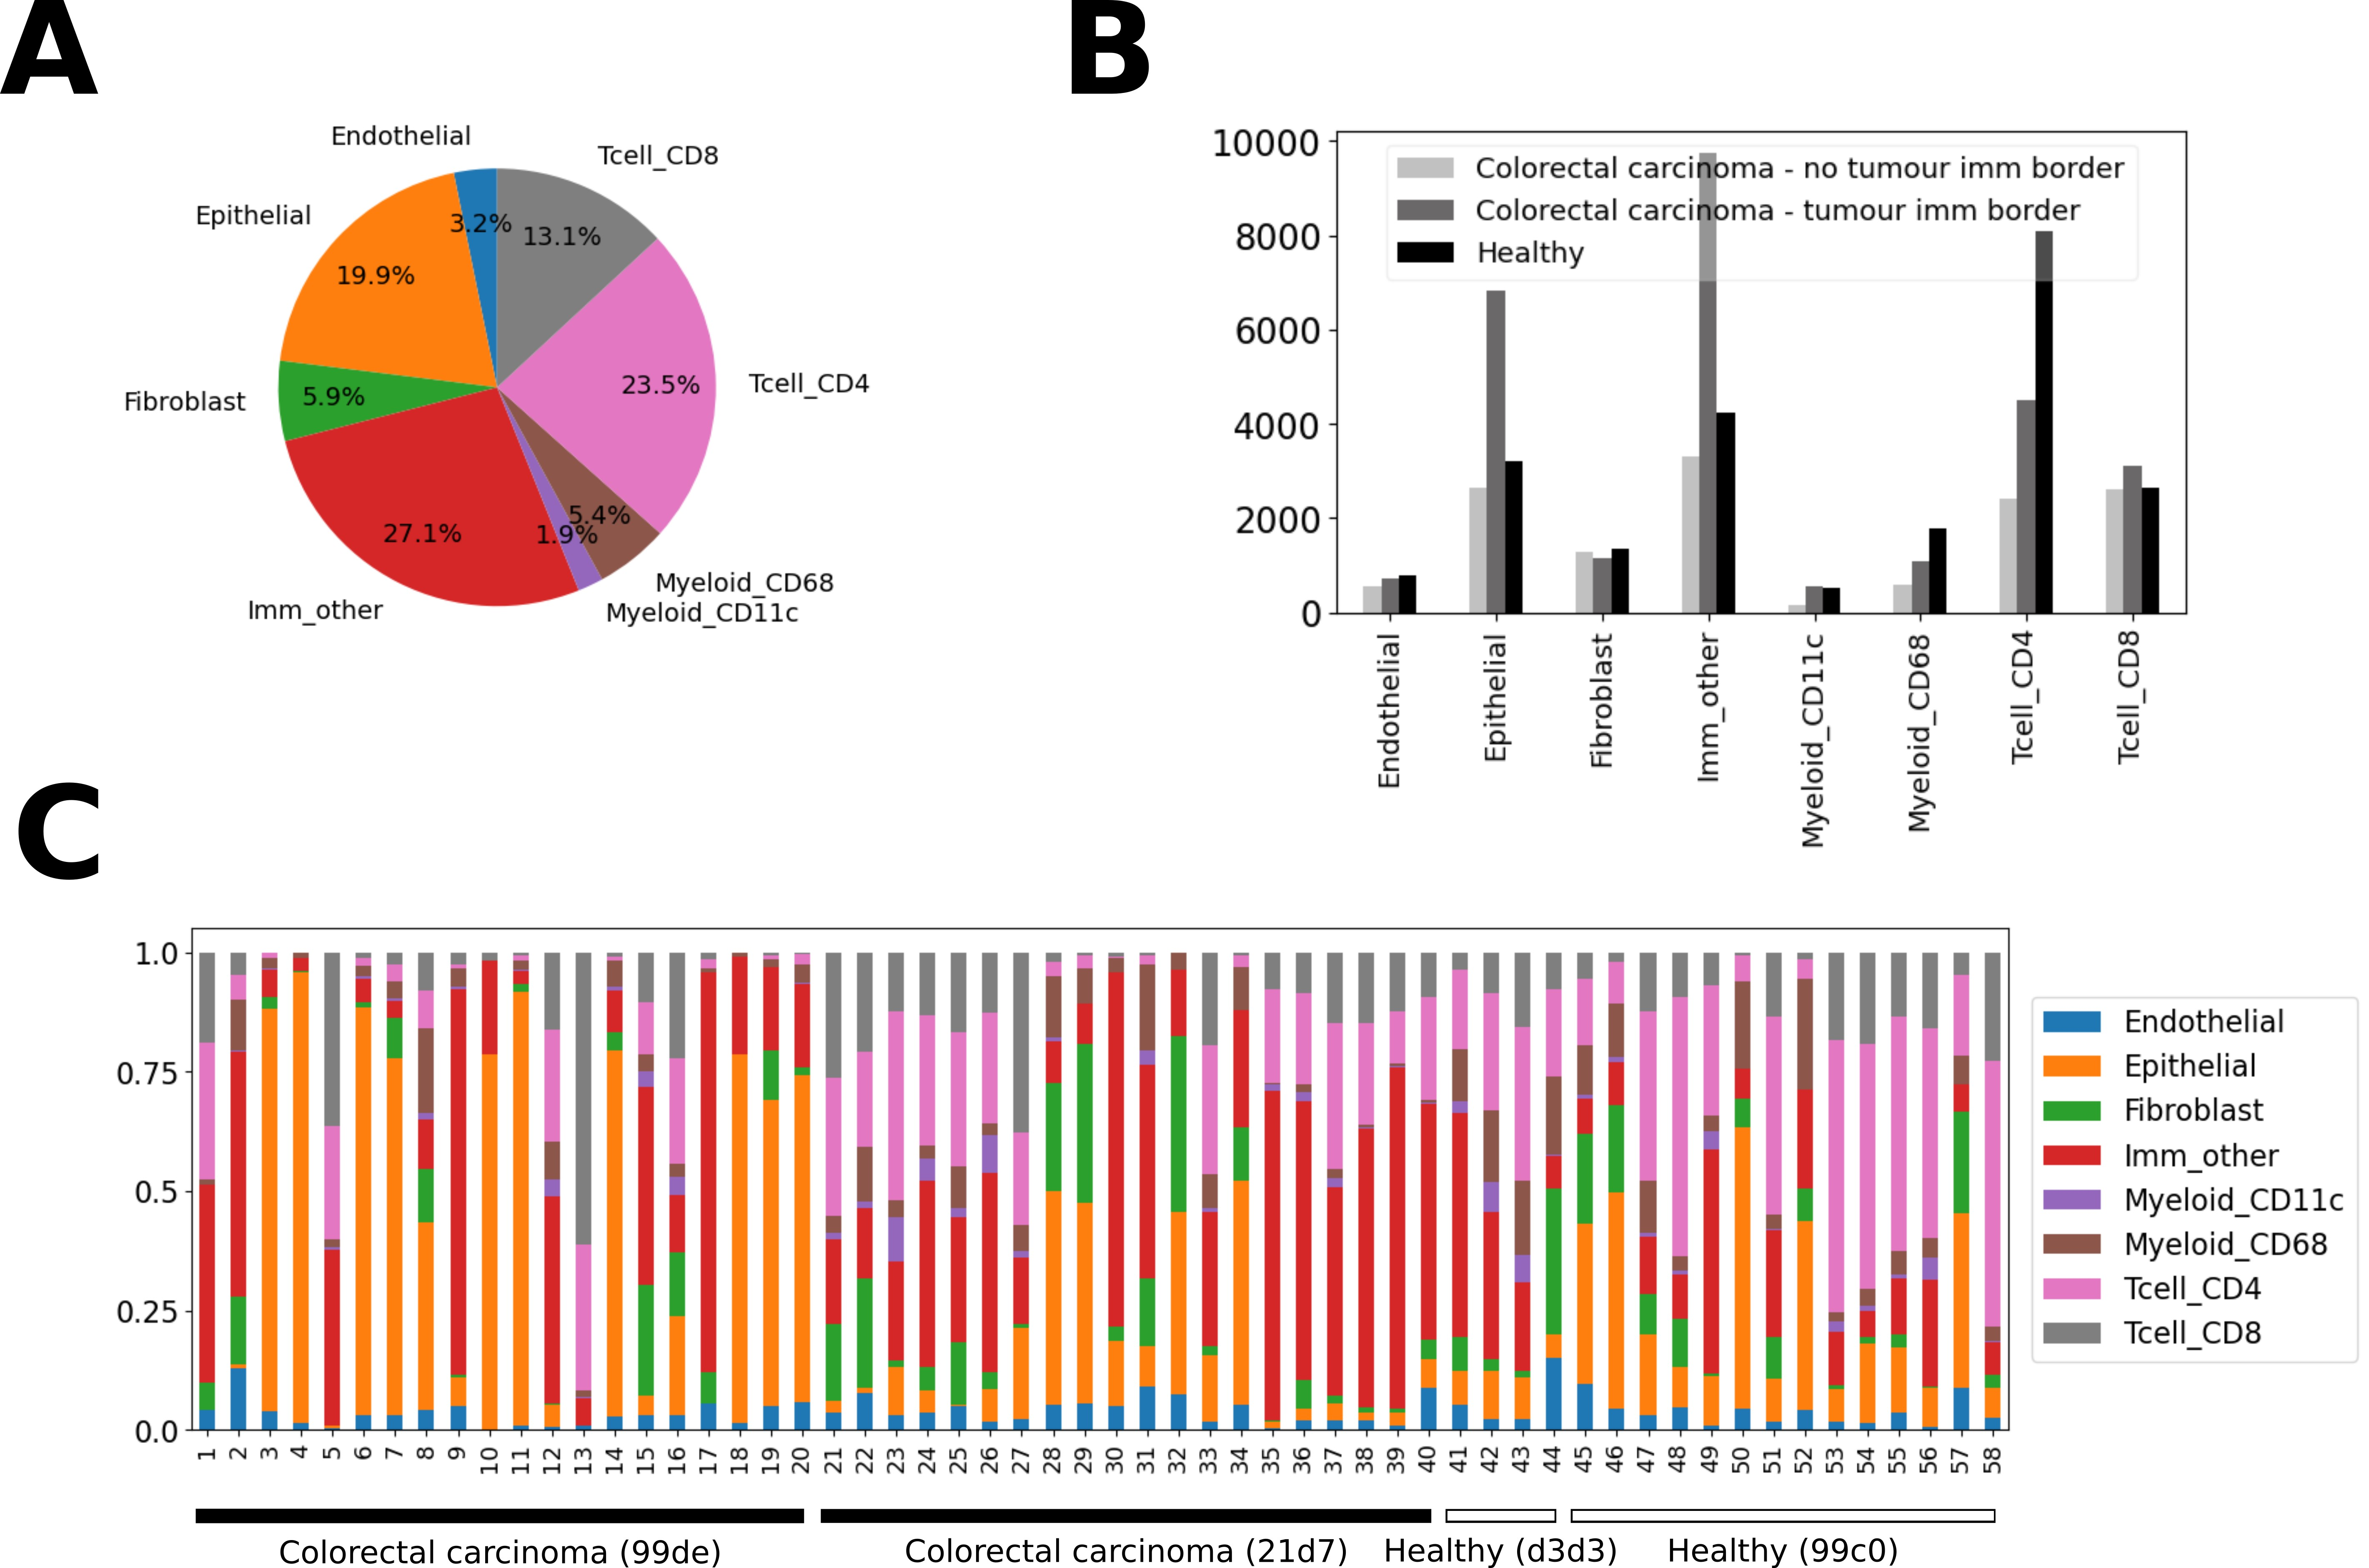
\includegraphics[width=16cm]{fig_cell-type_frequency_distributions}
    \caption{\textbf{Cell-type frequency distributions.} (A) Proportion of cell-types across all samples, donors and conditions. (B) Cell-type counts grouped by condition and tumour-immune border presence as defined by \cite{Hartmann-2021}. (C) Proportion of cell-types within a sample for all samples}
    \label{fig:freq}
\end{figure}


Next, the collective dataset (pooled single-cell data across all samples, conditions and donors) was analyzed for general variance, clustering or expression patterns. Mean feature expression was calculated for each feature yielding unique expression patterns for each of the annotated cell-types (Fig. \ref{fig:exploration}A).

Next, variation sources were examined via PCA. The first two principal components of PCA on the pooled single-cell data showed no distinct separation of cells by sample, condition or donor whereas cells of the same cell-type did cluster (Fig. \ref{fig:exploration}B). This indicates low batch effects from these sources and high variance due to cell-types. However, endothelial, myeloid CD68, myeloid CD11c and fibroblast cell-types did not separate as clearly as CD4\textsuperscript{+}, CD8\textsuperscript{+} T cells, endothelial and 'other immune cells'. Since the cell-type accounted for most of the variation, the original pooled feature space of the single-cell data was used for further collective dataset analysis like NCEM. Additionally, performing UMAP on the neighbourhood graph, based on the first 10 principal components of the PCA, showed clustering of the cite{Hartmann-2021} annotated cell-types, where again CD4\textsuperscript{+}, CD8\textsuperscript{+} T cells, endothelial and 'other immune cells' clustered more clearly than endothelial, myeloid CD68, myeloid CD11c cells and fibroblasts.

\begin{figure}[p]
    \centering
    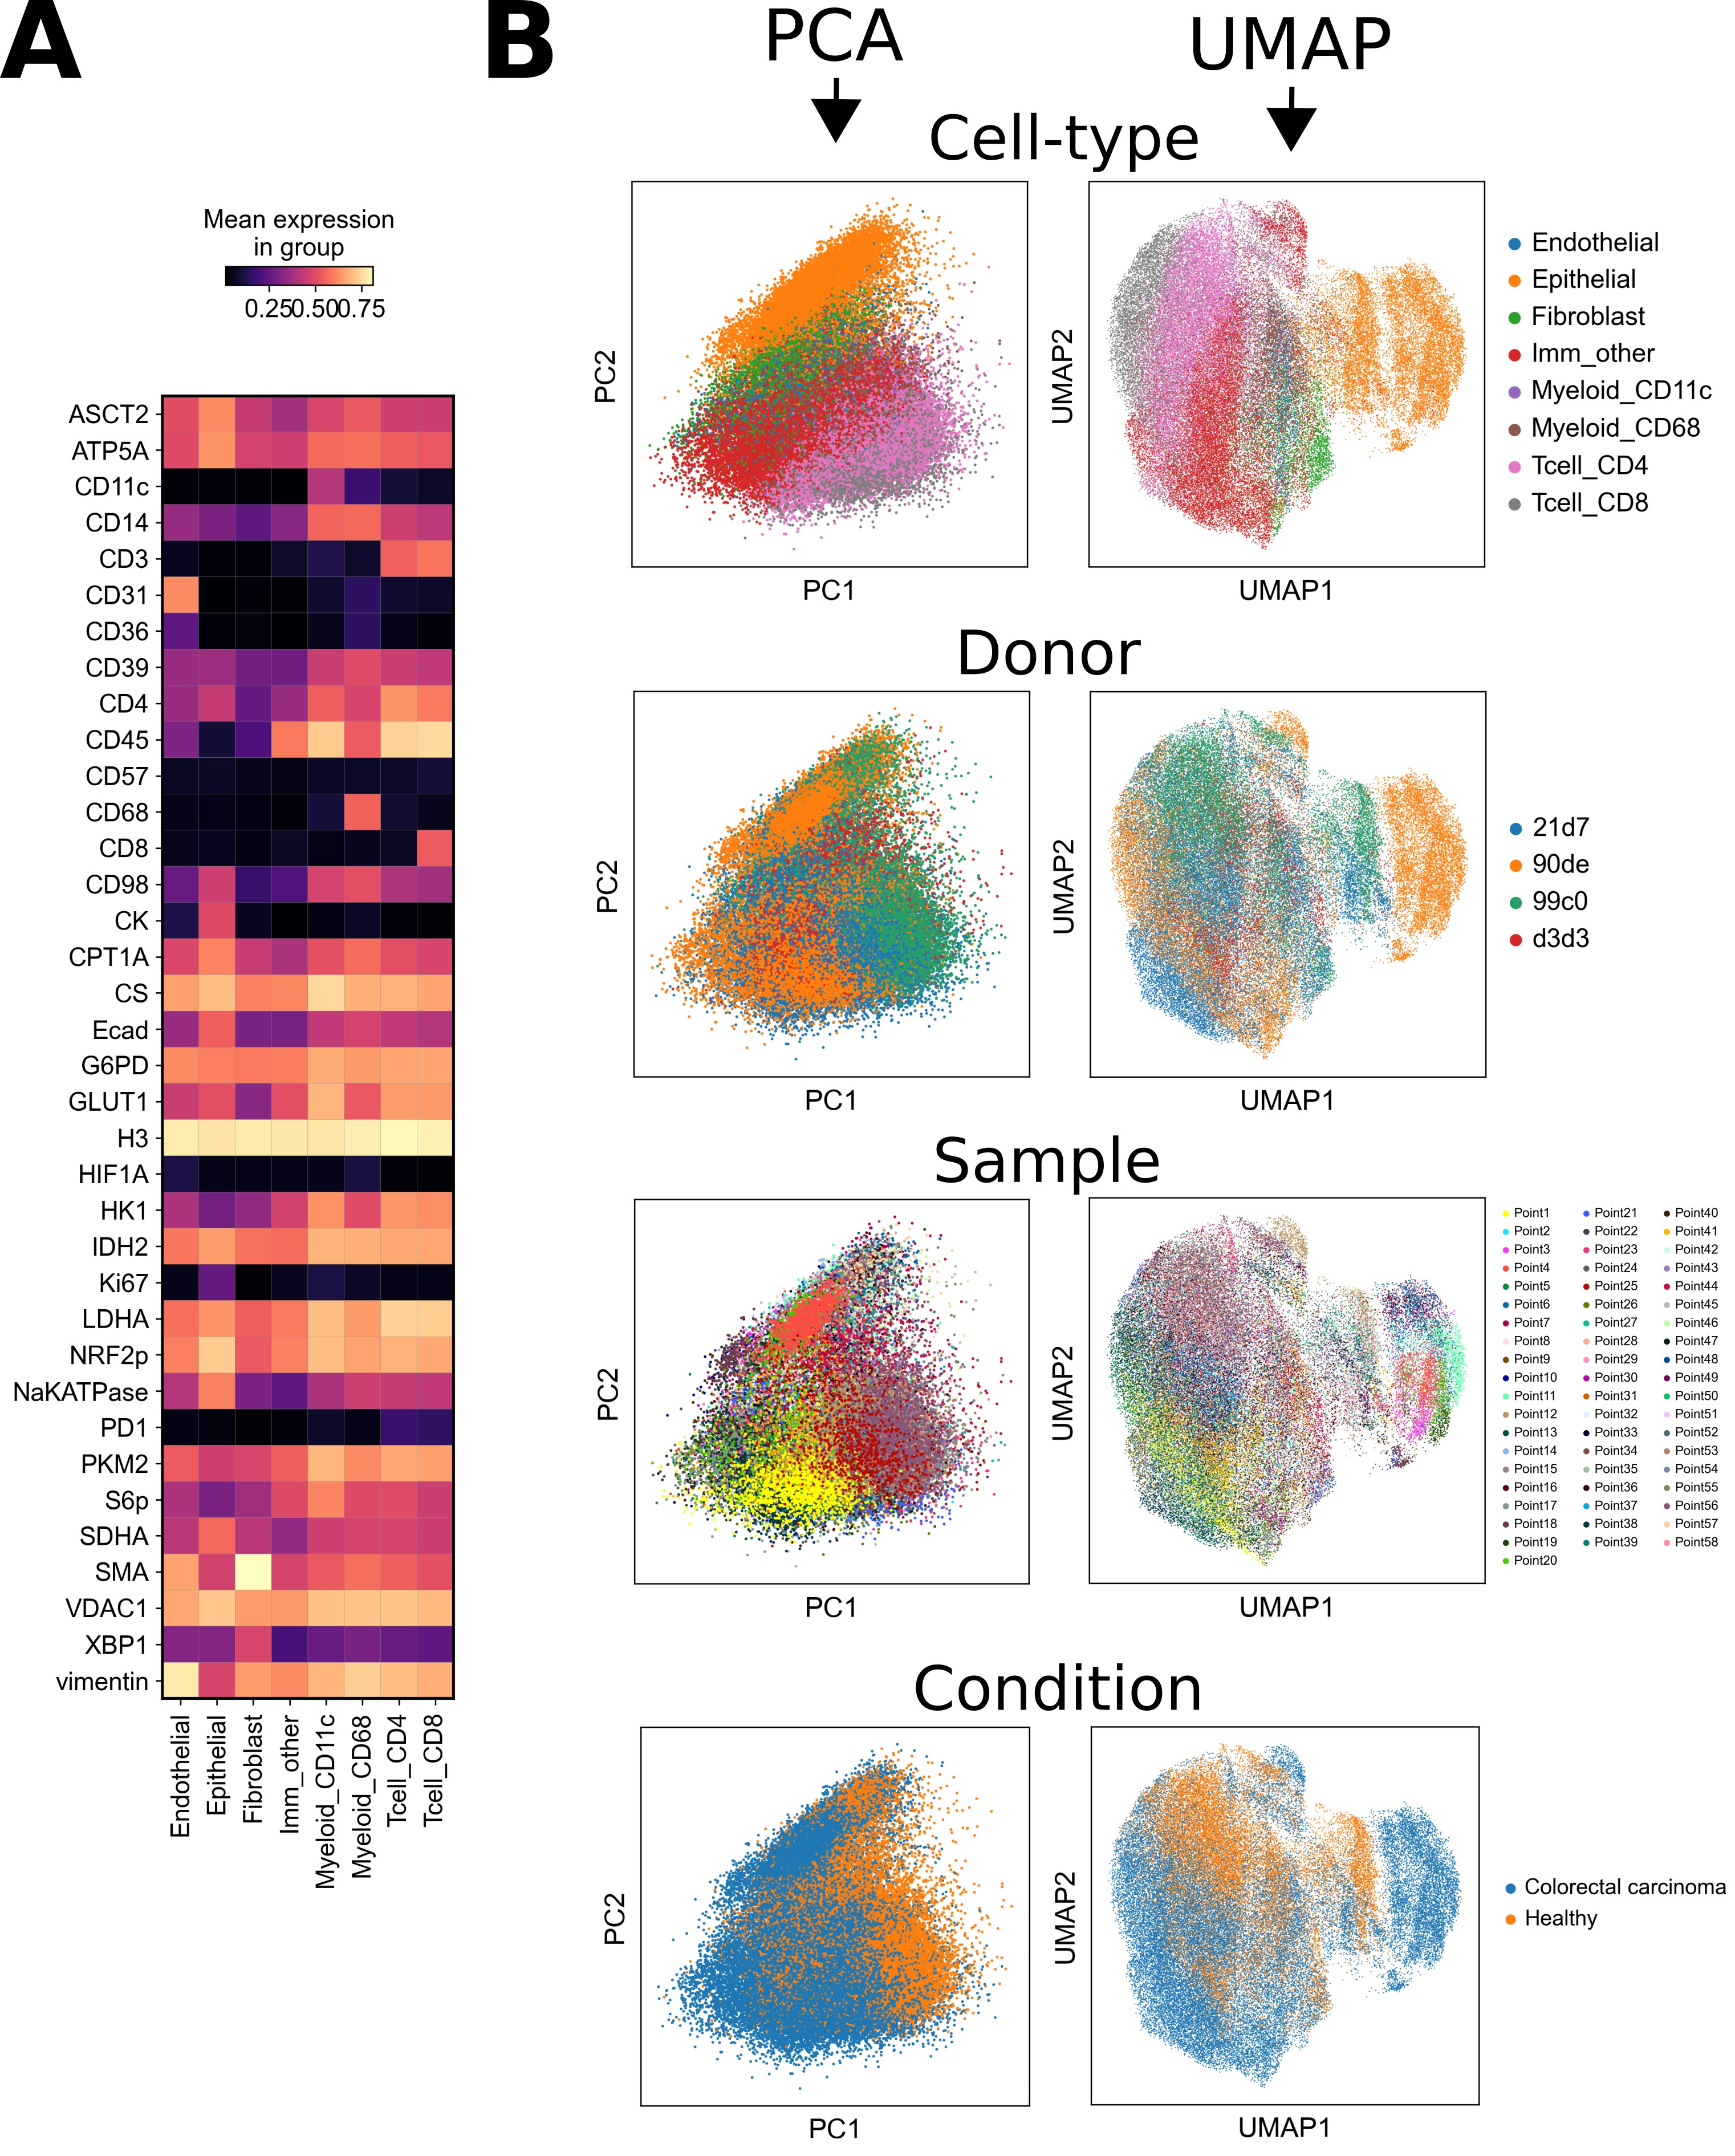
\includegraphics[width=16cm]{fig_global_expression_pca_umap}
    \caption{\textbf{Data exploration of the Hartmann-2021 dataset on pooled single-cell data across samples, donors and conditions.} (A) Feature expression mean was calculated by cell-type and lineage marker across all samples, donors and conditions. (B) Juxtaposed 2-dimensional representation of PCA and UMAP dimensionality reduction coloured by cell-type, donor, sample and condition. The neighbourhood graph and UMAP  were calculated using the first 10 principal components}
    \label{fig:exploration}
\end{figure}


The specific expression profiles of major immune cell lineage markers from the original paper were recovered via the mean expression per cell-type (Fig. \ref{fig:lineage-recovery}A,C). On the UMAP space (Fig. \ref{fig:lineage-recovery}B), it was expected that the expression of the lineage markers would enrich or deplete according to their cell-type. This was observed with the exception of markers CD11c, CD68 and CD31, corresponding to cell-types whose clustering was less clear in the UMAP space. Furthermore a set of 12 highly variable features were obtained that were not part of the lineage-marker set (Supplementary table \ref{tab:sup-hvargs}).

\begin{figure}[h!]
    \centering
    \includegraphics[width=16cm]{fig_lineage_profile_recovery}
    \caption{\textbf{Lineage specific expression profiles of provided cell-type annotation by Hartmann-2021.} (A) The expression mean of major immune lineage specific markers was calculated by cell-type and lineage marker across all samples, donors and conditions. (B) The neighbourhood graph and consecutive UMAP embedding was performed using the first 10 principal components and then coloured by cell-type and (C) by the major immune lineage markers.}
    \label{fig:lineage-recovery}
\end{figure}

\pagebreak



\section{Exploration and characterization of colorectal carinoma and healthy samples}

Next, two arbitrary samples were chosen for an exemplary analysis on an image-level basis.  "Point23" was chosen from the colorectal carcinoma samples with a tumour-immune border (defined as per Hartmann-2021). "Point49" was chosen from the healthy colon samples.

PCA and UMAP were performed on the cancer sample to examine how much cell-type accounts for variation. The first two principal components only accounted for epithelial cell-type separation. UMAP clustered CD4\textsuperscript{+}, CD8\textsuperscript{+} and 'immune other' cells in addition to epithelial cells (Fig. \ref{fig:explor-cancer}A). Plotting the expression of major immune lineage markers under the cell segmentation area revealed the expected spatial distribution and enrichment linked to their cell-type (Fig \ref{fig:explor-cancer}B). In addition, highly variable genes of the sample which differed from the lineage markers were calculated (Supplementary table 1) and the expression under the segmentation mask of CD98, Ki67 and NaKATPase are plotted (Fig \ref{fig:explor-cancer}C). CD98 was expressed towards the cancerous epithelial cells with depletion in the epithelial cells. Ki67 was sparsely expressed in apparently arbitrary cell-types. NaKATPase was found to be enriched towards the cancerous epithelial cells.

\begin{figure}[p]
    \centering
    \includegraphics[width=16cm]{fig_cancer_sample_exploration}
    \caption{\textbf{Exploratory data analysis of the colorectal cancer sample "Point23".} (A) Segmentation mask, PCA and UMAP coloured by cell type. UMAP was performed on the neighbourhood graph of the first ten principal components. (B) Major immune lineage marker expression under the segmentation mask. (C) Expression of highly variable features were are not lineage markers.}
    \label{fig:explor-cancer}
\end{figure}

To contrast the characterization of the colorectal carcinoma sample, PCA and UMAP were performed on the healthy "Point49" sample (Fig. \ref{fig:explor-healthy}). Similar to the colorectal carcinoma sample, the first two components' variation only accounted for the clustering and distinction of the epithelial cell type (Fig. \ref{fig:explor-healthy}A). Upon performing UMAP on the neighbourhood graph of the first 10 principal components, the 'immune other' cell type clustered and separated from the remaining cell-types (Fig. \ref{fig:explor-healthy}B). The latter cell-types clustered but didn't separate.

Highly variable genes in the collective dataset (pooled single-cell data) were found in either the highly variable genes set of the colorectal carcinoma sample "Point 23" or the healthy sample "Point49". Accordingly, plotting the expression under the segmentation mask wasn't necessary (Fig. \ref{fig:explor-healthy}C).

\begin{figure}[p]
    \centering
    \includegraphics[width=16cm]{fig_cancer_sample_exploration}
    \caption{\textbf{Exploratory data analysis of the healthy sample "Point49".} (A) The segmentation mask coloured by cell-type and the first two dimensions of PCA and UMAP. (B) The segmentation mask of coloured by the expression levels of the major immune lineage markers. (C) Highly variable features not found within the lineage marker feature set.}
    \label{fig:explor-healthy}
\end{figure}

\pagebreak


\section{Spatial statistical analysis of cell-type distributions}

In order to investigate CCC it is important to analyze the spatial context of the the image samples on a cell-type level. This can validate or uncover tissue and niche structures as well as hint towards cell signaling on different spatial organizational levels like juxtacrine and paracrine signaling between cell types.

First the connectivity graphs of both the colorectal carcinoma sample "Point23" and the healthy sample "Point49" were calculated (Fig. \ref{fig:spatial-stats}A) by setting the neighbourhood size to a radius of 35 px (~14µm), as was calculated by \cite{Fischer-2022} to yield the best predictive performance on this dataset (explained variance, R\textsuperscript{2}) as a hole and by cell-type.

Given the anatomy of the colon, we expected a clear epithelial wall to be present in both carcinoma and healthy samples and therefore the epithelial cells to cluster. Similarly, we expected immune cells and possibly fibroblasts to aggregate close to the epithelium forming the lamina propria. Ripley's L statistic was computed to analyse the relative distribution of cells of the same annotated cell type (Fig. \ref{fig:spatial-stats}B). Indeed in both the carcinoma and healthy samples, CD4\textsuperscript{+} T cells and other CD45\textsuperscript{+} immune cells showed the highest score indicating higher relative clustering. In the carcinoma sample the CD4\textsuperscript{+} T cells had the highest score the followed by other CD45\textsuperscript{+} T cells. In the healthy sample the order was reversed. In both samples epithelial cells also showed a relatively high Ripley's L score ranked 3rd in both conditions. Furthermore, the clustering coefficient centrality scores were computed, which measure the degree of node clustering in the spatial graph for cell-type annotations. The obtained scores in the colorectal carninoma sample showed higher clustering scores in immune cells and epithelial cells compared to remaining non-immune cells (endothelial and fibroblasts) (Fig. \ref{fig:spatial-stats}C). Clustering coefficients in the healthy sample showed fibroblasts to be less clustered than the rest of the cells.

Once the clustering patterns were analyzed, relative spatial proximity between cell-types was measured via neighbourhood enrichment analysis and co-occurrence. Neighbourhood enrichment yielded in both carcinoma and healthy conditions higher values in the diagonal than other cell-type pairs (Fig. \ref{fig:spatial-stats}D). In the colorectal carcinoma sample epithelial and 'other CD45\textsuperscript{+} immune cells' showed noticeably high intra-cell-type enrichment scores indicating their respective clustering. Similarly in the healthy sample showed high enrichment of between same cell-type pairs CD4\textsuperscript{+}, CD8\textsuperscript{+} T cells and CD11c\textsuperscript{+}, CD68\textsuperscript{+} myeloid cells. Additionally CD4\textsuperscript{+} and CD8\textsuperscript{+} T cells showed to be mutually enriched. CD11c\textsuperscript{+} and CD68\textsuperscript{+} myeloid cell pairs also showed high enrichment scores. With respect to cell-type proximity to the epithelial wall, the co-occurrence score was computed for all cell-types given the presence of epithelial cells for increasing distance (Fig \ref{fig:spatial-stats} E). Applied on the colorectal carcinoma sample, it was shown that fibroblasts were more likely to be found near epithelial cells at close distance (400 px $\approx$ 156 µm) than at further distance (600 px $\approx$ 234 µm). Epithelial cell co-occurence showed high vales in this interval which declined with distance, further showing epithelial cell clustering. CD4\textsuperscript{+} and CD8\textsuperscript{+} T cells showed a constant co-occurence score while other CD45\textsuperscript{+} cells co-occurrence increase with distance to epithelial cells. Co-occurence scores on the healthy colon sample showed high values in the close range (100 px $\approx$ 39 µm) for epithelial, endothelial, CD11c\textsuperscript{+} and CD68\textsuperscript{+} myeloid cells. These scores quickly declined to a plateau at (400 px $\approx$ 156 µm). Epithelial cells had noticeably higher co-occurrence scores in at 39 µm radius indicating clustered behaviour.

\begin{figure}[p]
    \centering
    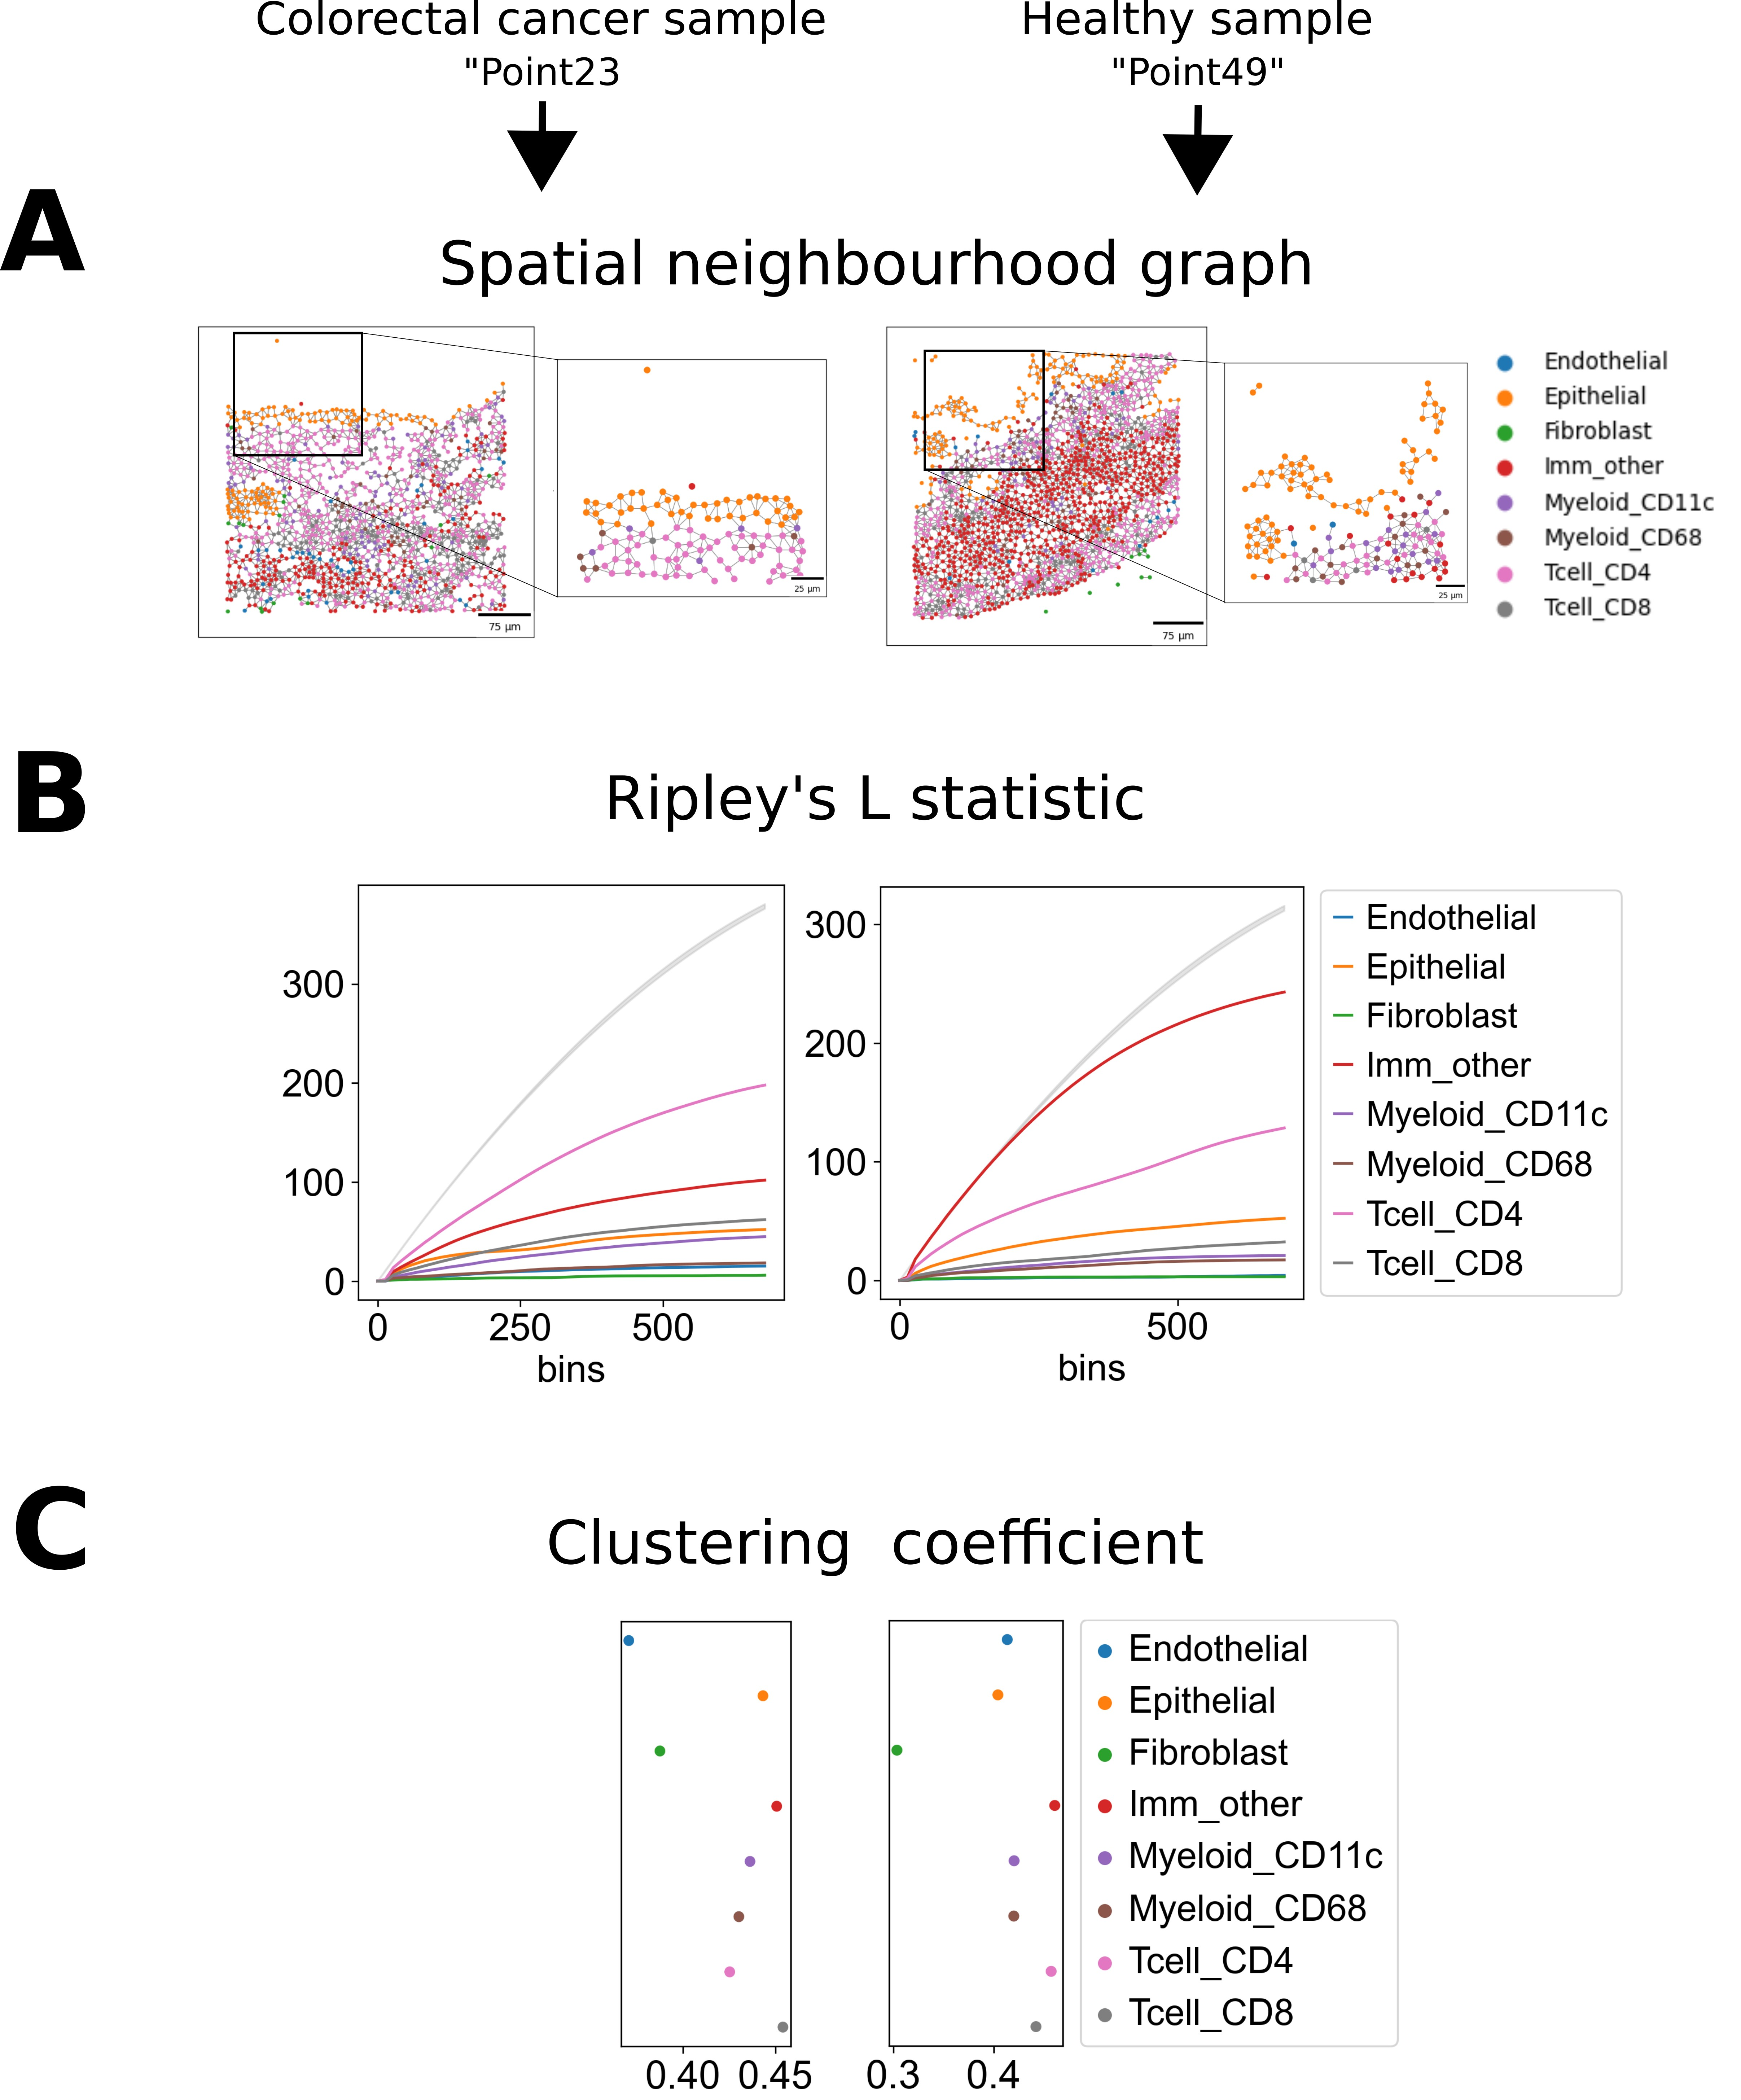
\includegraphics[width=16cm]{fig_cancer_vs_healhty_spatial-statistics_1}
\end{figure}

\begin{figure}[p]
    \centering
    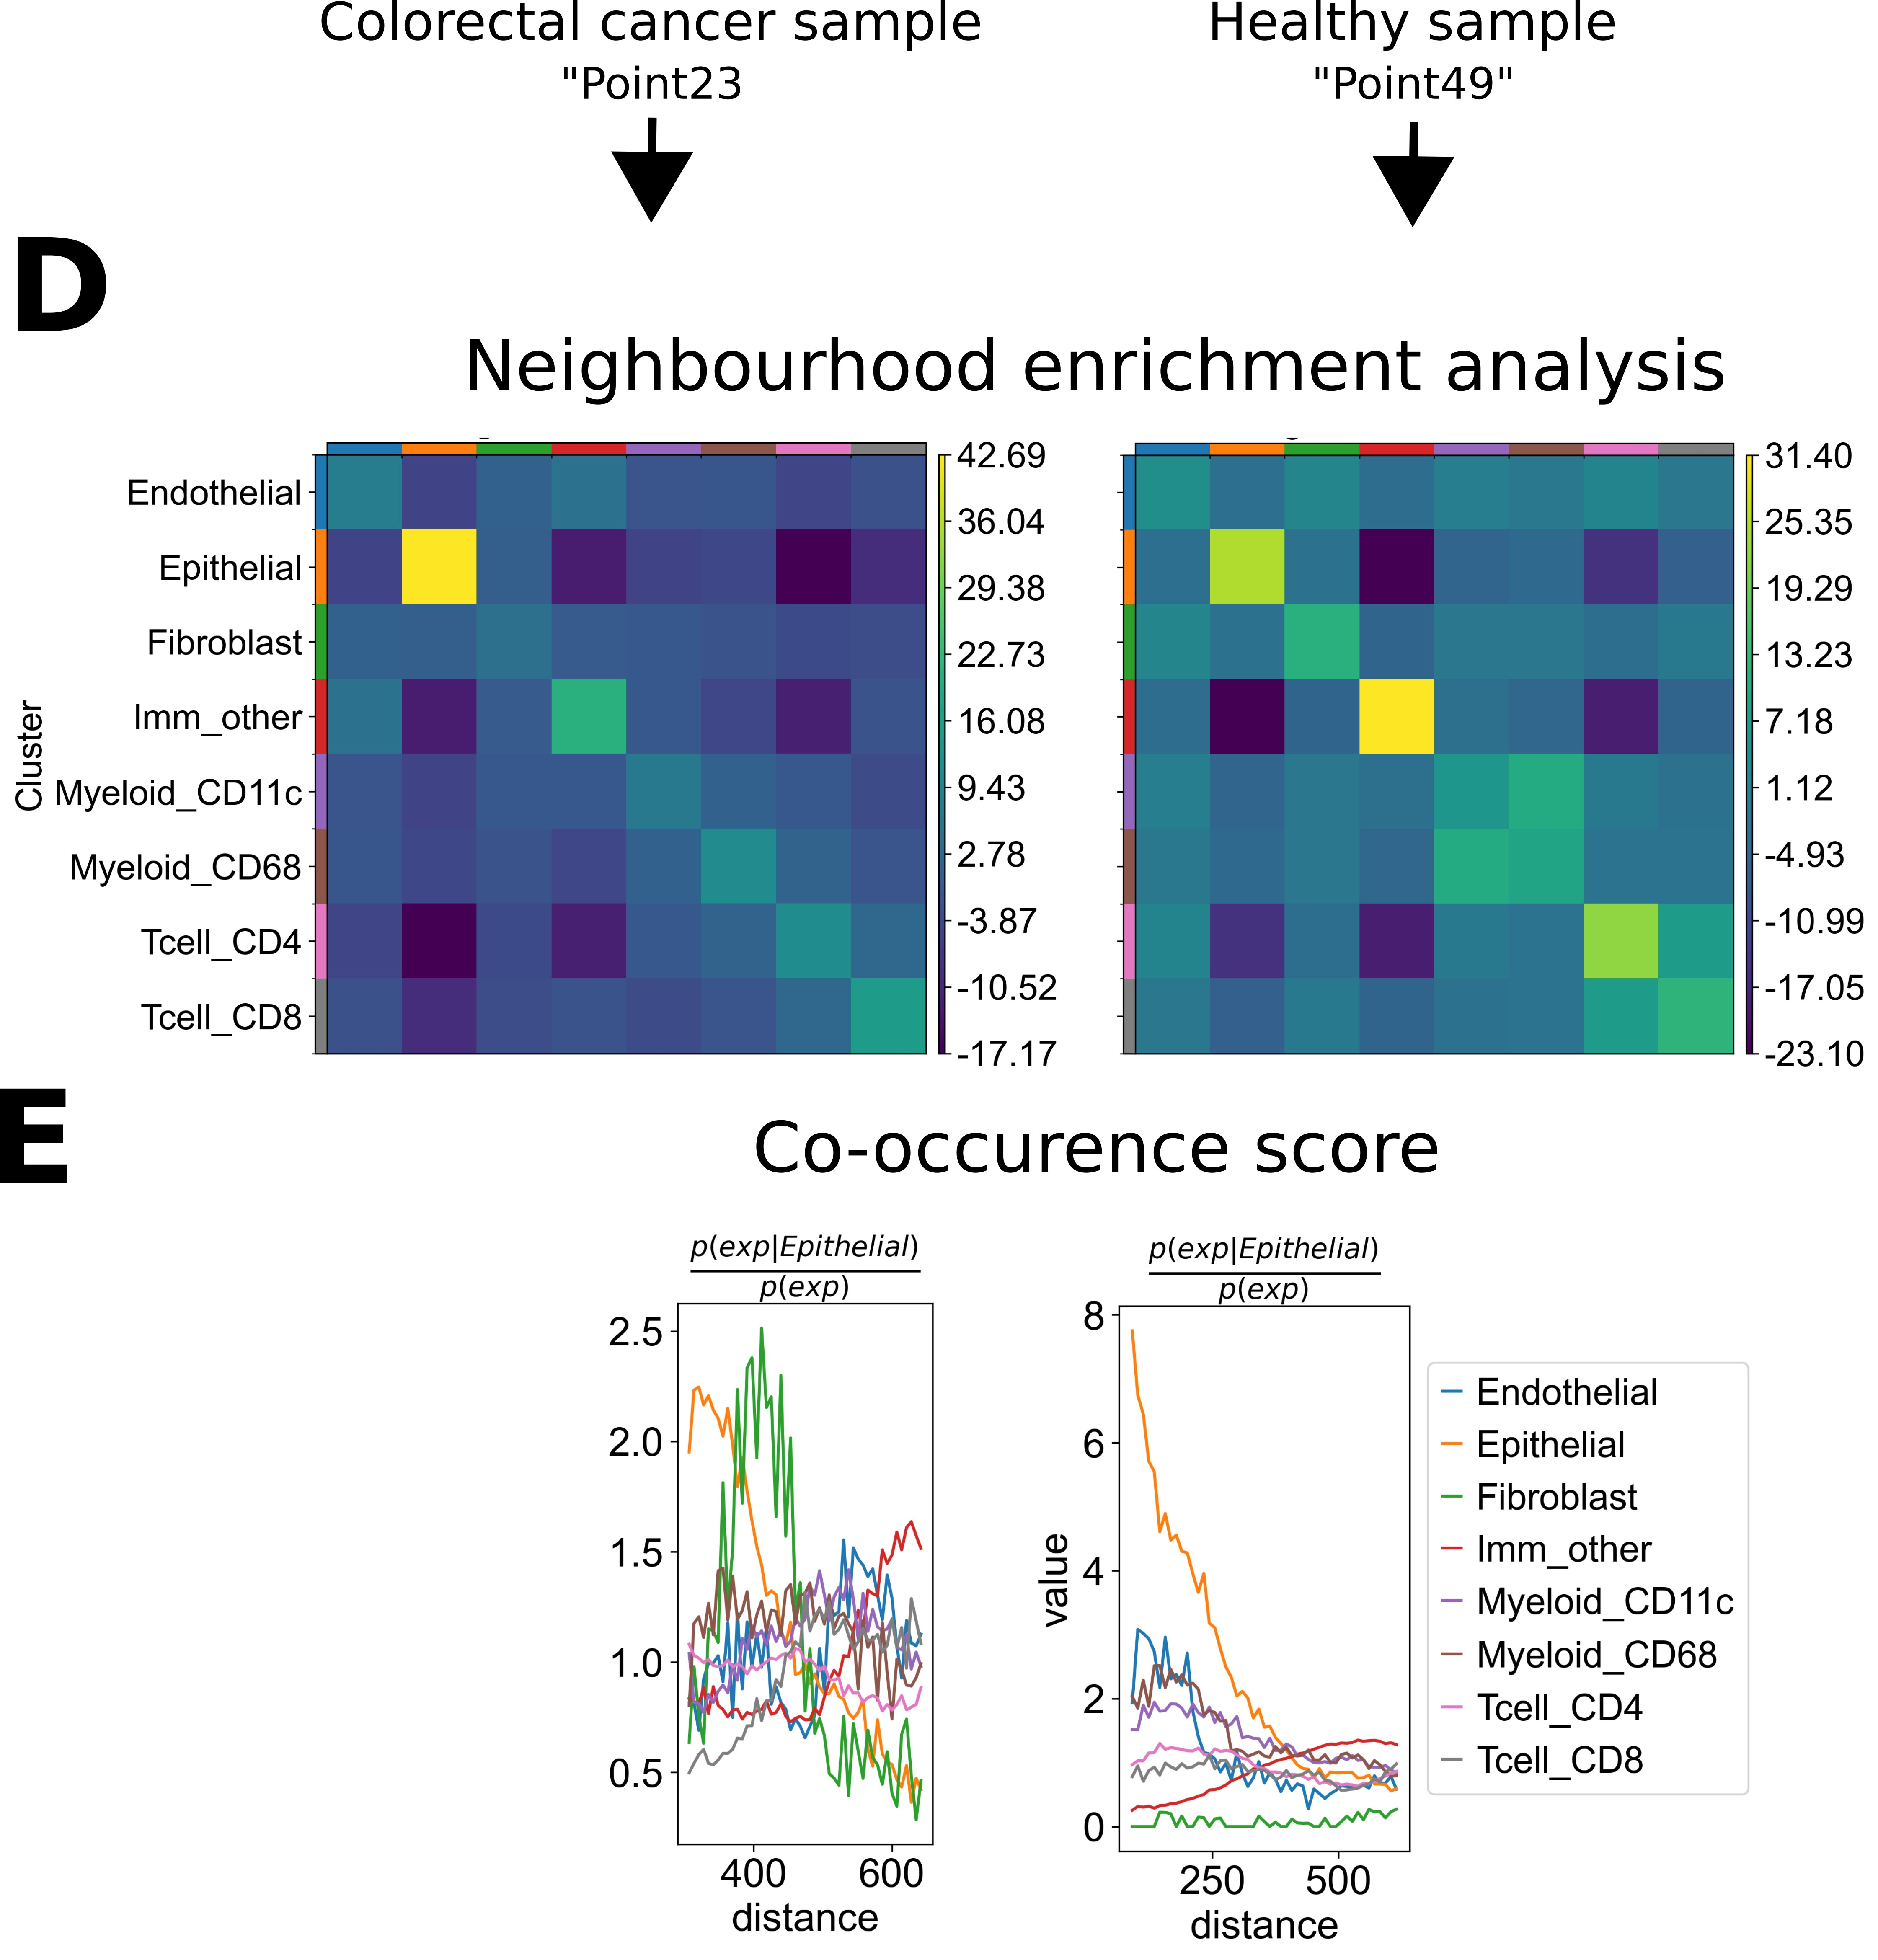
\includegraphics[width=16cm]{fig_cancer_vs_healhty_spatial-statistics_2}
    \caption{\textbf{Spatial statistical analysis of annotated cell-type distribution on the spatial connectivity graph.} Colorectal carcinoma sample "Point23" localized on the left and the healthy sample "Point 49" on the right. (A) Spatial connectivity graph calculated using a radius threshold of 35 px (~14 µm). (B) Ripley's L spatial distribution statistic (C) Clustering coefficient scores computed via Squidpy (D) Neighbourhood enrichment analysis (E) Co-occurence score.}
    \label{fig:spatial-stats}
\end{figure}



\section{Spatially variable features}

In order to obtain a fuller context on a spatial level, the analysis of spatial cell-type distribution was complemented with analysis of spatially variable features on the colorectal carcinoma sample "Point23" and healthy colon sample "Point49". This was achieved via the Morans I auto-correlation statistic (Supplementary fig. \ref{tab:sup-moran}), which describes the level of dispersion and clustering of a feature across space. It was predicted that the major immune lineage markers would score a Moran's I value closer to 1 since they should enrich in their in their corresponding cell-types according to their unique profile (Fig. \ref{fig:lineage-recovery}A). In addition, highly variable genes found previously were hypothesized to show some spatial patterning. Indeed, in the colorectal cancer sample, four of the ranked features by Moran's I score were from the lineage marker set (descending order: CK, CD45, CD11c, CD4) (Fig. \ref{fig:lineage-recovery}A, \ref{fig:explor-cancer}B). Furthermore, two of the top ranked features pertained to the previously calculated highly variable features (CD98, NaKATPase) (Fig. \ref{fig:explor-cancer}C, Supplementary table \ref{tab:sup-hvargs}) and four novel features were obtained (GLUT1, HK1, LDHA, PKM2) (Fig. \ref{fig:moran}). From the top ten ranked features by Moran's I score on the healthy colon sample, 7 pertained to the major immune lineage marker set (descending order: CK, CD45, CD11c, vimentin, E-cadherin, CD14, CD3) (Fig. \ref{fig:lineage-recovery}A, \ref{fig:explor-healthy}B), 3 formed part of the preiously calculated highly variable features (CD98, Ki67, NaKATPase) (Fig. \ref{fig:explor-healthy}C, Supplementary table \ref{fig:sup1}) and no novel features with distinct expression in space were found.

\begin{figure}[h!]
    \centering
    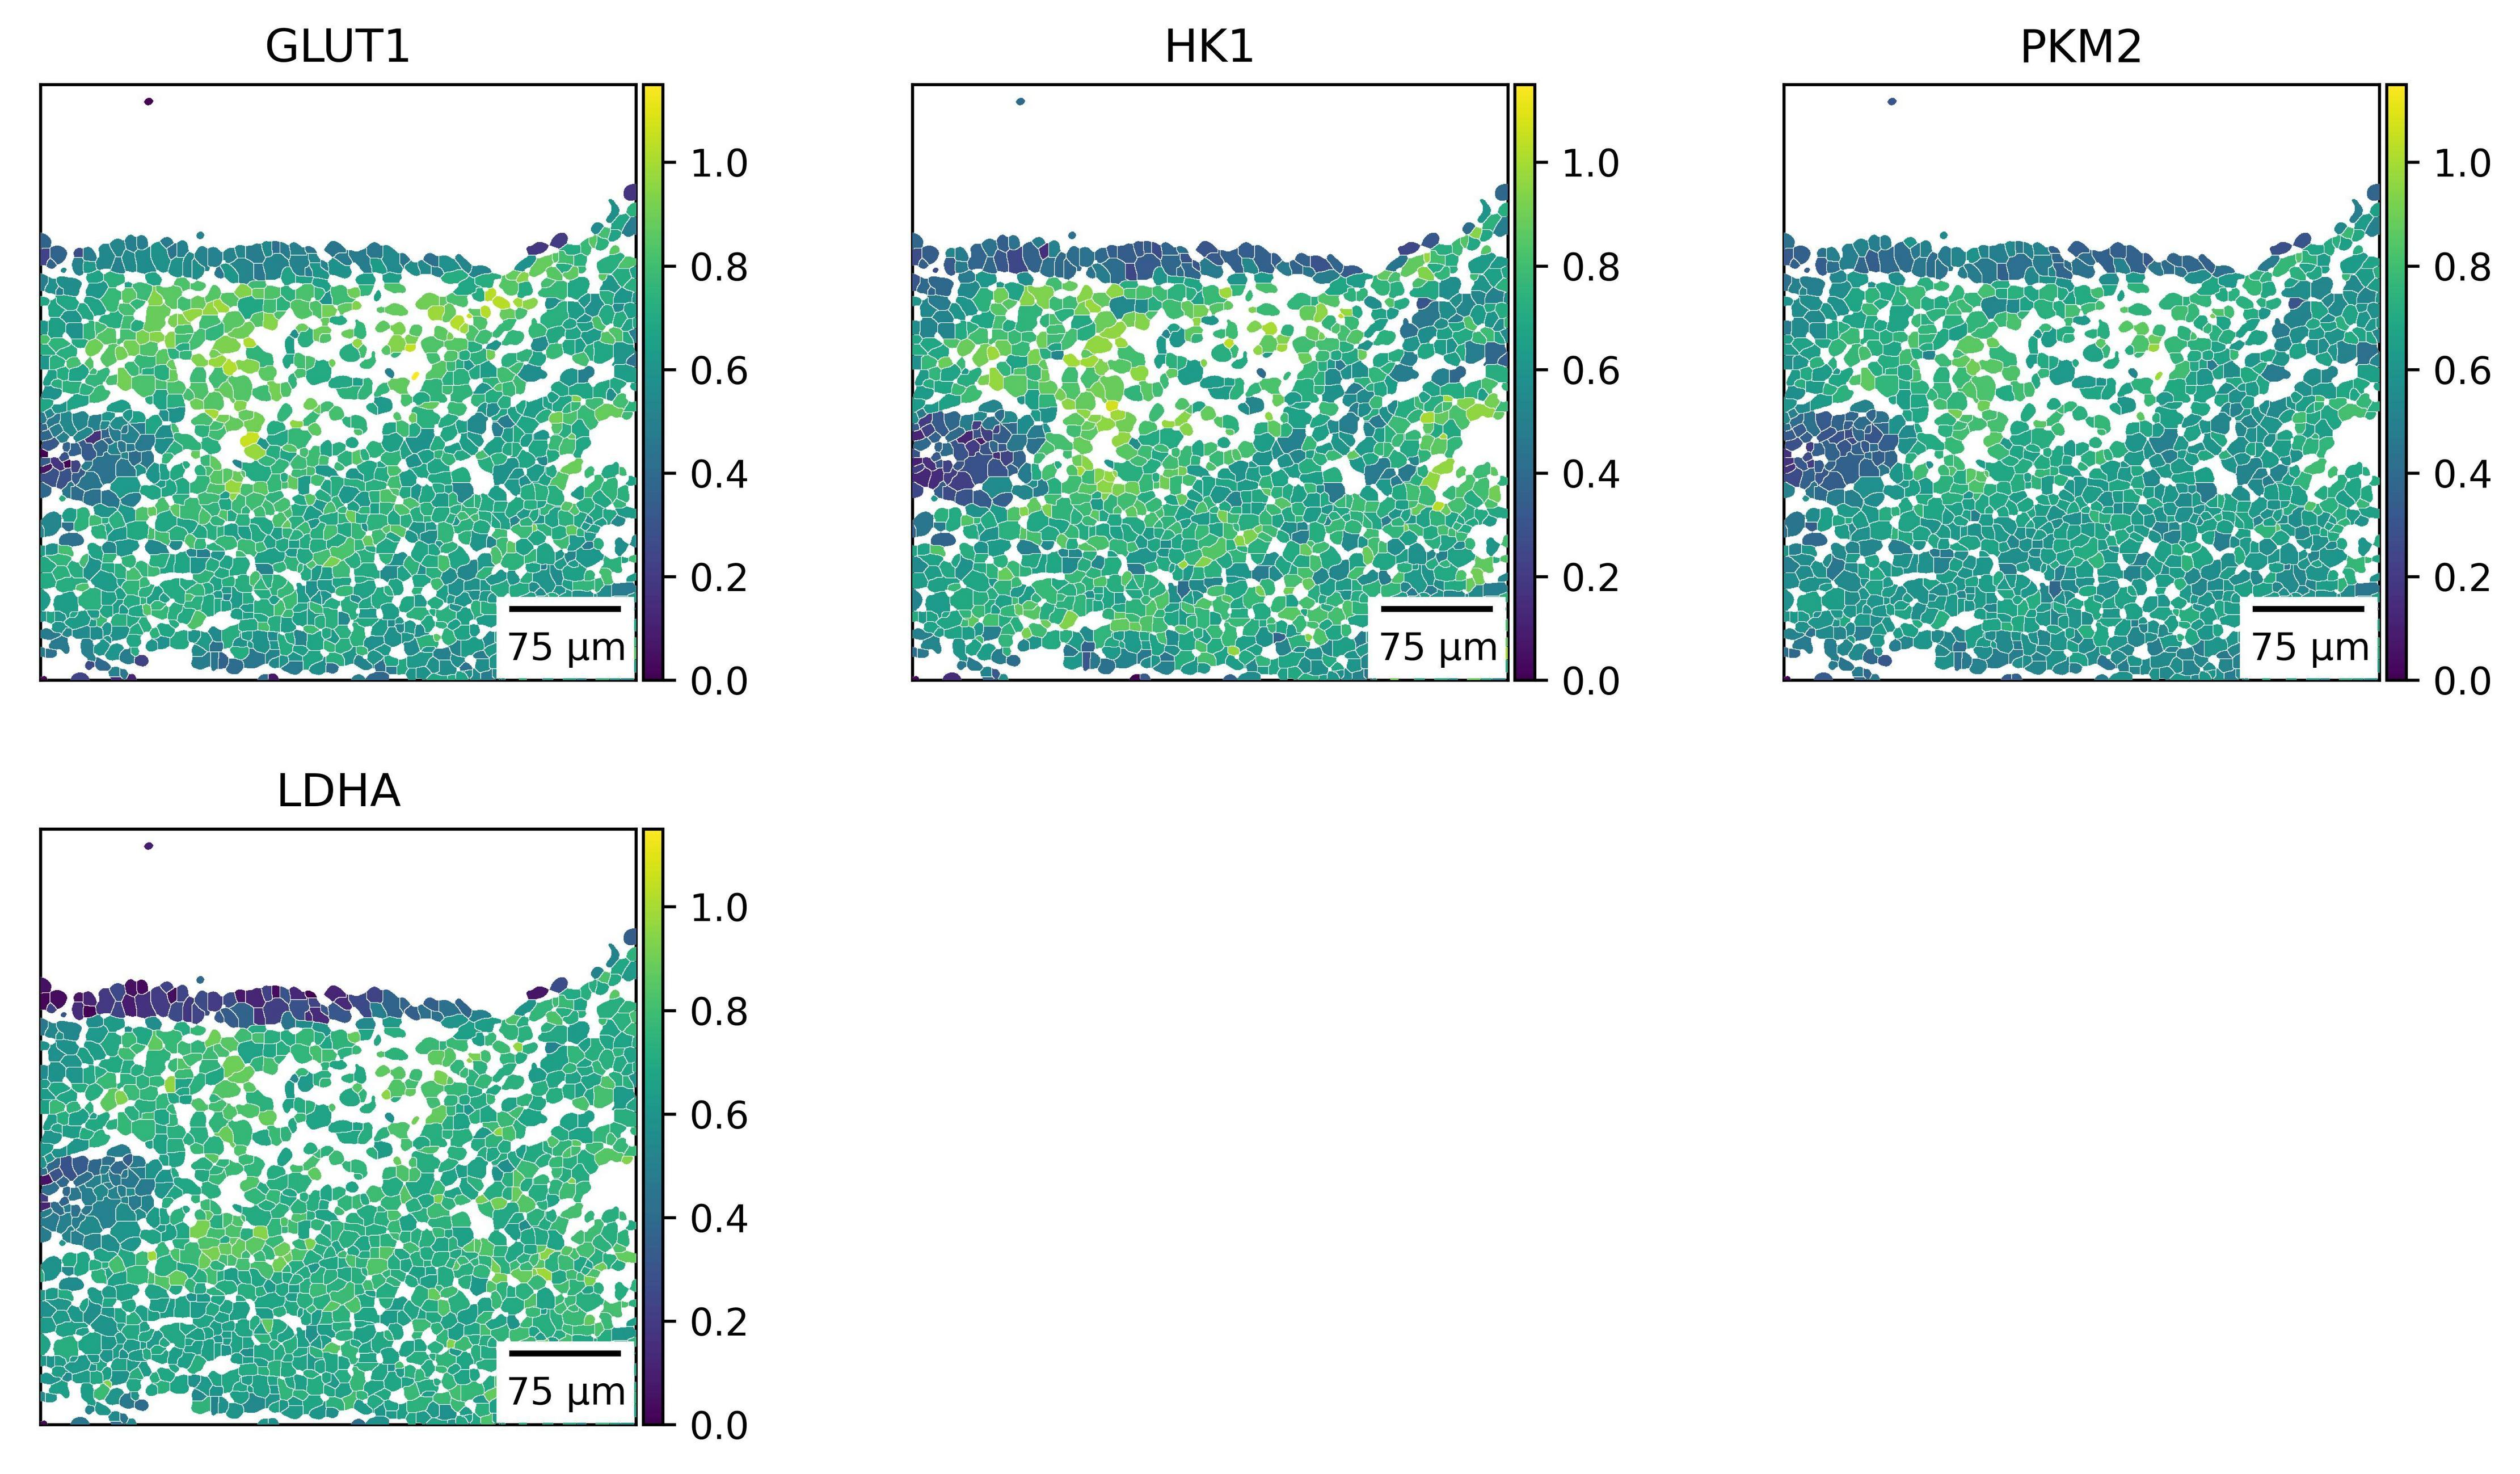
\includegraphics[width=16cm]{fig_moransi}
    \caption{\textbf{Novel top ranked features by Moran's I score on colorectal carcinoma sample "Point23"**. Segmentation mask coloured of "Point23" coloured by the expression of features scoring top 10 in the Moran's I analysis and were not part of either the previously investigated immune lineage markers or the highly variable features calculated for the present sample.} Colorectal carcinoma sample "Point23" localized on the left and the healthy sample "Point 49" on the right. (A) Spatial connectivity graph calculated using a radius threshold of 35 px (~14 µm). (B) Ripley's L spatial distribution statistic (C) Clustering coefficient scores computed via Squidpy (D) Neighbourhood enrichment analysis (E) Co-occurence score.}
    \label{fig:moran}
\end{figure}

\pagebreak


\section{Cell-type-based sender-receiver effects calculation via NCEM interaction-terms}

Once the dataset had been characterized on the spatial and non-spatial level, the CCC methods were applied.

First, the NCEM linear model was applied to the entire dataset to obtain the interaction term coefficients, also referred to as sender-receiver effects. They are obtained asymmetrically for each sender-receiver cell-type pair and are specific to the directional interaction (dimensions: receiver cell-type x sender cell-type x features). Alongside the interaction term coefficients, FDR-corrected significance values for each interaction term were obtained for the performed Wald test.

To summarize the three-dimensional tensor, two approaches were followed. First, \cite{Fischer-2022}s approach was followed, in which the number of significant interaction terms after hypothesis testing are quantified via the L1-norm of the FDR-corrected p-value tensor. The user can set the significance threshold and an additional threshold for minimum number of obtained significant features (Fig. \ref{fig:ncem}A). Sender epithelial cells showed noticeably high interaction values on receiving CD4\textsuperscript{+} T cells. Sender CD4\textsuperscript{+} T cells showed high values when paired with CD11c, CD68 myeloid cells and other CD45\textsuperscript{+} immune cells. Other CD45\textsuperscript{+} immune cells showed high valued-interactions both as sender and receiver cells.

The second approach was aimed to be less reliant on discrete values based on a significance threshold and allow for the value of the interaction term to shape the summary statistic. This was achieved via the application of the L2-norm on the significance filtered interaction term tensor. The user can define a range- or standard-deviation-based threshold value for the used interaction terms as well as a threshold for the final L2-norm obtained values. The latter threshold can be a high-pass threshold or a percentile-based threshold. Similar to the previous significance-based approach, this approach showed a high interaction term value for the sender epithelial and receiver CD4\textsuperscript{+} cells. In contrast to the previous method, for the sender epithelial cells, a high value for the interaction with CD11c\textsuperscript{+} myeloid cells was observed. Another dissimilarity was the obtained high value for the endothelial-epithelial cell-types pair. When observing the sender effect of CD4\textsuperscript{+} T cells, their interaction coefficients on all other cell-types were not as high as in the previous approach relative to all the values in the distribution. In other words, the relative effect of CD4\textsuperscript{+} T cells on all other cells was decreased in the L2-norm approach in comparison to the significance based approach. The same relative effect reduction could also be observed on both the sender effect of 'other CD45\textsuperscript{+} immune cells' on all other cell-types and the receiver effect of 'other CD45\textsuperscript{+} immune cells' by all other immune cells. The only noticeably high values that were constant in both approaches were the 'other CD45\textsuperscript{+} immune cells' effect on CD11c\textsuperscript{+} immune cells and the receiving effect of 'other CD45\textsuperscript{+} immune cells' by CD8\textsuperscript{+} T cells.

Since the linear NCEM model is reliant on correct cell-type annotation it was hypothesized that simulating false cell-type annotation due to upstream artifacts or uncertainty in processing steps would greatly impact the output of the model. Fischer et al.'s approach to testing linear NCEM's robustness against cell segmentation error was limited to the exchange of neighbouring nodes' vectors. These, however, are often of the same cell type. Hence, it was attempted to expand on this robustness analysis by applying linear NCEM on shuffled cell-type annotations in varying fractions of random cells (fractions: 0\%, 0.1\%, 1\%, 10\%, 50\% and 100\%; shuffling repetitions for each fraction: n=15) (Fig. \ref{fig:ncem}B). As expected, the explained variance ($R^2$) already decreased in the interval between none and 1% fraction shuffling. The decrease of $R^2$  between the shuffling of 1% of the cells and 10% accounted for most of the explained variance by the model, as 50% shuffling reached the same level of $R^2$ as completely randomized cell-type annotation.

\begin{figure}[p]
    \centering
    \includegraphics[width=14cm]{fig_ncem_interactions_and_shuffling}
    \caption{\textbf{Application of linear NCEM.} (A) Sender-receiver effects obtained via two approaches. Two interaction term summary approaches (1) Quantifying the significant features per cell-type pair. The FDR-corrected p-value tensor was filtered by a significance threshold of 0.05 and the consecutively the L1-norm was calculated (Left) (2) Applying the L2-norm on the interaction terms coefficients tensor, previously filtered by a significance threshold of 0.05 (Right). (B) NCEM application on shuffled cell-type annotations by different fractions of random cells whose annotations were randomized. For each box, the center-line defines the median of the explained variance ($R^2$), the height of the box represents the inter-quartile range (IQR) and the whiskers denote the 1.5 * IQR.}
    \label{fig:ncem}
\end{figure}

\pagebreak


\section{Analysis of spatial dependencies via MISTy}

The next step was to apply MISTy to the dataset. MISTy is a predictive machine learning framework which defines "views" as spatial contexts that are to be used to predict the feature expression of the index cells. In our specific case, to not deviate too much from the NCEM concept of neighbourhoods, only one view was defined apart from the standard "intra-view". This "para-view", was constructed by adding the feature expression of cells within a certain radius 35 px (~14µm) of the index cell in a weighted manner (gaussian kernel). MISTy was run using an ensemble random forest algorithm for F().  Three types of data were collected (1) the gain of explained variance ($R^2$) achieved by comparing the $R^2$ of the model with solely the "intra-view" and the $R^2$ of the model that includes  both the "intra-view" and the "para-view" (Fig. \ref{fig:misty}A) (2) the contribution of each view to the metamodel in form of the learnable weight parameters (Fig. \ref{fig:misty}B) and (3) the improvement of the prediction of target features in the index cell via a leave-one-out procedure of predictor features in the "para-view" (Fig. \ref{fig:misty}C). MISTy was run on an individual sample level and the results where aggregated via the mean and standard deviation summary statistics.

The gain in $R^2$ of the aggregated results showed very high standard deviation, often accounting for its entire effect. SMA, PD1 and H3 were the top ranked proteins that contributed to the gain in $R^2$ by ~2.5 fold increase. Next, the results on the individual colorectal carcinoma sample "Point23" were examined yielding CD8, H3 and CD11c to be the top ranked proteins improving $R^2$ by ~3 fold. When examining the healthy colon sample "Point49", PD1, CD11c and Ki67 were the proteins that improved the $R^2$ the most by over a 4 fold increase.

The contributions of each view to the metamodel for each protein showed, as expected, that most of the contribution (consistently >50\%) comes from the "intra-view" or from the intrinsic index cell feature signaling when regarding the aggregated results. Some of the proteins that showed the highest contribution of the "para-view" were CD11c, CD8 and HIFA. In the colorectal carcinoma sample HIFA and KI67 showed a higher contribution of the "para-view" than the "intra-view". In the healthy colon sample, only CD8 showed more than half of the contribution via the "para-view". 

The feature importance results of MISTy showed sparse results in the aggregated, carcinoma sample and healthy sample results. CK was a predictor with noticeably many of the highest values across the three latter conditions. CK showed high predictive importance for target S6p, SDHA, SMA, VDAC1 in the colorectal carcinoma and healthy samples but only SDHA and SMA showed high results were high for the aggregated results. CPT1A was only high in the aggregated results. E-cadherin and citrate synthase (CS) were only high for the colorectal cancer sample and healthy sample respectively. Predictor CK was hight for ASCT2 and ATP5A in the aggregated resulst and colorectal cancer sample while only ASCT2 was high in the healthy sample. Predictor CD11c showed many high values in the colorectal carinoma and healthy samples.

\begin{figure}[hb!]
    \centering
    \includegraphics[width=8cm]{fig_misty_intra-para_r2-improvements}
\end{figure}

\begin{figure}[p]
    \centering
    \includegraphics[width=16cm]{fig_misty_intra-para_contributions-and-importances}
    \caption{\textbf{MISTy analysis of spatial dependencies by defining the "intra-" and "para-view"}. The results are shown for three categories (1) the aggregated results over all samples (Top), (2) the results on the individual colorectal carcinoma sample "Point23" (Middle) and (3) the results on the individual healthy colon sample "Point49" (Bottom). (A) Gain in variance explanation when comparing the MISTy model solely with the "intra-view" and the MISTy model including both the "intra-" and the "para-view". (B) The learnable parameters of the metamodel for each view for every feature. (C) The importances contrast heatmap. The importance of each feature to the prediction of the individual targets from the "intra-view" are subtracted from the importances calculated for the "intra-view".}
    \label{fig:misty}
\end{figure}

\pagebreak


The obtained results via MISTy were not suitable for comparison with the sender-receiver effects calculated via NCEM due to format disparity. Since the overarching goal was to to lay the groundwork for future benchmarking and evaluation of CCC methods, an approach was devised to adapt the MISTy workflow to yield comparable output. The approach consisted of transforming the input of MISTy from the feature expression matrix to the one-hot encoding matrix of the own index cells, yielding a comparable output (Fig. \ref{fig:misty_cell-types}). In essence, the prediction approach changed to predicting the index cell-type based on the neighbourhood cell-type weighted abundance. The "intra-view" was bypassed to avoid illogical prediction of cell-type within the index cell. The "para-view" was additionally modified to use a constant kernel (sum of neighbourhood cell-types across cells).

The variance explained $R^2$ was not a contrast in this case, since there was no "intra-view" to subtract. Hence it was not considered. Neither were the learnable weights results considered, since the contribution was modeled to come from the "para-view" solely.

The importances output showed no positive importance for any cell-type pair for the aggregated statistic (Fig. \ref{fig:misty_cell-types}). For the colorectal carcinoma sample, predictor endothelial cell-type showed interaction values for targets "other immune CD45\textsuperscript{+} cell", fibroblasts and CD4\textsuperscript{+} T cells.  In contrast, when examining the results on the healthy colon sample, predictor CD11c\textsuperscript{+} myeloid cells had a positive interaction value for epithelial, "other immune CD45\textsuperscript{+}", and CD4\textsuperscript{+} T cells. Also, predictor cell-type CD4\textsuperscript{+} T cells showed positive interactions with target CD11c\textsuperscript{+} myeloid, endothelial and fibroblast cells.

\begin{figure}[h!]
    \centering
    
\includegraphics[width=8cm]{fig_misty_cell-types_importances}
    \caption{\textbf{MISTy workflow modified to achieve a comparable output to NCEM.} Cell-types were used as input for MISTy. Three different result categories were shown: (1) aggregated results across all samples (Top), (2) application of MISTy to colorectal carcinoma sample "Point23" (Middle) and (3) MISTy applied to healthy colon sample "Point49" (Bottom). (A) The importances heatmap of the "para-view" for each target and predictor pair.}
    \label{fig:misty_cell-types}
\end{figure}

\chapter{Discussion}
	


In the present study spatial cell-cell communication methods NCEM and MISTy were applied and evaluated for benchmarking on the \cite{Hartmann-2021} colorectal cancer MIBI-TOF dataset. Applying the linear NCEM model output the interaction terms coefficients, also refered to as sender-receiver effects. These were further summarized via two approaches: (1) quantifying the amount of significant features per sender-receiver cell-type pair and (2) calculating the L2-norm of interaction terms matrix which had previously been filtered by a significance threshold. There were some distinct interactions found in both summarizing statistics, for example the interaction between sender epithelial and receiver CD4\textsuperscript{+} T cells. However, there were also dissimilarities present as the interaction between epithelial and CD11c myeloid cells was not as high in approach 1 compared to approach 2, relative to all interactino values. Also, in the first approach, other CD45\textsuperscript{+} immune cells showed high interactions with most cell-types both as sender and receiver whilst in approach 2, most of these interactions were diluted. None of these interactions can be validated due to the lack of ground truth. Common upstream errors and artifacts are one of the major challenges in the spatial-omics field. For example, incorrect feature detection attribution to its corresponding cell due to imprecise cell-segmentation can lead to incorrect cell-type labeling. We analyzed the sensitivity of the linear NCEM model towards cell-type labels by shuffling the cell-type of varying fractions of randomly selected cells. The high sensitivity even at low shuffling fractions like 10\%, which is common in spatial-omics processing, indicates that variation in the pre-processing steps will have a great effect on linear NCEM output and that both the spatial technology used to obtain the data and the pre-processing steps effectuated before NCEM application must be assessed carefully to account for false annotation.

The flexibility of MISTy to define the views and independence of cell-type annotation was the key reason for its application. Additionally, defining the "para-view" as the weighted sum of the neighbourhood features promised more robustness from upstream artifacts and segmentation errors. However, a different set of problems were encountered upon application compared to NCEM. First, MISTy natively runs on on individual samples and aggregates their results via summary statistics like the mean and standard deviation. The standard deviation obtained for the increase of explained variance ($R^2$) was very high and virtually always in the range of the own mean value. Also, the top ranked features for this result varied greatly when inspecting individual samples (e.g. colorectal carcinoma and healthy colon). The metamodel learnable parameters for each view, also referenced to as contributions, showed continuously higher contributions from the "intra-view" than the "para-view" with exceptions in the individual sample resolution. The higher HIFA and Ki67 contributions from the "para-view" effect found in the colorectal carcinoma sample "Point 23" which were not found in the healthy colon sample "Point49" and the aggregated results could be a hint towards the effect of the cancer. However, making a statement would be speculative due to the lack of ground truth. The feature importances results calculated as the difference between the "juxta-view" and the "intra-view" showed CK and CD11C to be relevant predictors.  with ASCT2, ATP5A, E-cadherin, CPT1A, CS, SDHA, SMA, VDAC1 and S6p. Target features E-cadherin and citrate synthase were specific to the colorectal carcinoma sample. E-cadherin has a key role in tumour metastasis \cite{Beavon-2000}. Disregulation of citrate synthase has been found to be linked to tumour malignancy and the Warburg effect\cite{Lin-2012}. The discrepancy between results of individual images and the aggregated result was observed with features like CPT1A , which was specific to the aggregated result, and S6p and VDAC1, which were high in the colorectal cancer and healthy samples but not in the aggregated result.

The second challenge was the lack of comparable output with linear NCEM's output. To this aim, the MISTy workflow was adapted to use the one-hot encoding of the index cell-types as input and the intra-view was bypassed. As such, the model would predict the index cell-type based on the count of neighbouring cell-types. The result type with comparable format to NCEM were the importances between the cell-type predictor-target pairs. For the aggregated results, no importances were found, while the individual examples showed that endothelial was a predominant predictor in the colorectal carcioma sample and CD4\textsuperscript{+} T-cells and CD11c\textsuperscript{+} myeloid cells were predominant in the healthy colon sample.

The application of MISTy showed the need for a better way to integrate different samples, donors and conditions. Alternatively, the user must have a precise comprehension about the biology and experimental setup to apply MISTy in a tailored manner and make any statements based on MISTy's output. MISTy's flexibility allowed for shaping of the output to our specific purposes. This came at the cost of low interpretability. Again, validation of the results was not possible due to the lack of ground truth.

In contrast to MISTy, NCEM models the sample or batch directly into the linear model. This could be practical to integrate samples. However, accounting for conditions in this way could influence the interaction terms and the final output. Similarly to MISTy, it is evident that the user must have a good understanding of the experimental setup to judge if all samples and conditions are to be included in the application of linear NCEM on a colletive dataset.

In order to critically assess these methods, the dataset was also statistically characterized on the spatial and single-cell level. Cell-type frequency distribution showed a high variability in cell-type frequencies across all samples and also between conditions which may lead to unbalanced model training in NCEM and MISTy, especially the latter since it is applied on an individual sample basis. By summarizing the mean feature expression of cell-types across all samples, the major immune lineage profiles were recovered based on specific markers. PCA analysis, clustering and UMAP embedding did not separate these cell-types clearly, indicating possible upstream annotations errors or the need for better sample integration. Spatial statistics verified the clustering of epithelial cells and immune cells as per colon tissue structure. In addition, Moran's I autocorrelation analysis uncovered features with clustered expression distribution which differed from the lineage markers: GLUT1, HK1, pyruvate kinase M2 (PKM2) and lactate dehydrogenase A (LDHA) in the colorectal carcinoma sample "Point23". GLUT1, PKM2 and LDHA were spatially enriched in most cells except cancerous epithelial cells. They are key proteins in channels and enzymes in the energy metabolism, possibly indicating the activation of immune cells near to the tumour-immune border.

In the big picture, the study highlights the lack of a consensus on the approach to quantify cell-cell communication effects which needs urgent reevaluation to adapt to the latest approaches and technologies. Dependence of spatial CCC methods from upstream steps and artifacts was also a repeated challenge throughout the study which was shown to contribute to unaccounted variation. The high number of uncertainty sources leads to the necessity of the establishment of new protocols, redefinition of concepts  and the development of new methods that take the latter factors into account. The lack of ground truth will also continue to obstruct spatial single-cell benchmarking and evaluation.

To continue the investigation, the outlook includes the application of other spatial CCC methods with different approaches. Non-predictive approaches like DIALOGUE, COMMOT and possibly other non-spatial methods (e.g. CellChat) could leverage other cell properties. Methods that integrate prior-knowledge like ligand-receptor interactions have great potential (e.g. CellPhoneDB v3 or Giotto).

The optimal approach to CCC inference is unclear. Ligand-receptor and protein-protein interactions are essential to cell-cell communication. However, their complexity is not captured well by current spatial technology data. Spatial-transcriptomics measures mRNA, which is only a proxy for protein abundance. Spatial proteomics technologies have a lower-plexity and don't capture the entire landscape of post-translational modifications. Relevant dimentions which are only partially accounted for in current CCC methods are protein-complex subunits, ligand-receptor competition, allosteric regulation and distal endocrine signalling amongst others. On the other hand, data-driven approaches offer prior-knowledge agnostic insights. These in turn are difficult to interpret and their source can be source  can be unclear or less relevant to CCC. Hence, the best CCC approach could be a combination of both approaches to leverage the known effects behind CCC while incorporating other effects agnostically extracted from the data. In addition, CCC will substantially benefit of improving spatial-omics technologies.

Furthermore, the comparison and benchmarking of CCC methods and the effect of upstream steps should remain the focus of further efforts. In-silico simulated spatial data could be used to benchmark the methods. CCC methods could also be applied to other datasets from a diverse range of technologies and omics to evaluate the robustness and flexibility of the CCC methods towards different technologies and omics. Applying NCEM and MISTy on the PCA space could be analyzed for predictive performance improvement. 



\section*{Code availability}

All the analysis, code, conda environment data, figures, input and output data are publically available at \url{https://github.com/idf-io/SpatialPipe}.



\section*{Data availability}

The colorectal carcinoma MIBI-TOF dataset (Methods) is publicably available at \url{https://zenodo.org/record/3951613}.

%\chapter{Outlook}


\bibliographystyle{bib/cell}
\bibliography{bib/bibfile}
\addcontentsline{toc}{chapter}{Bibliography}

\chapter{Supplementary information}


\begin{table}[!h]
    \centering
    \caption{Highly variable genes on pooled data and subsampled data by condition}
    \begin{tabular}{llll}
    \hline
        \textbf{} & \textbf{Global} & \textbf{Colorectal carcinoma} & \textbf{Healthy samples} \\ \hline
        ASCT2 & ~ & ~ & ~ \\
        ATP5A & ~ & ~ & ~ \\
        CD11c & ~ & ~ & ~ \\
        CD14 & X & ~ & X \\
        CD3 & X & X & X \\
        CD31 & ~ & ~ & ~ \\
        CD36 & X & ~ & X \\
        CD39 & ~ & ~ & ~ \\
        CD4 & ~ & ~ & X \\
        CD45 & X & X & X \\
        CD57 & ~ & ~ & ~ \\
        CD68 & ~ & ~ & ~ \\
        CD8 & ~ & X & ~ \\
        CD98 & X & X & X \\
        CK & X & ~ & ~ \\
        CPT1A & ~ & ~ & ~ \\
        CS & ~ & ~ & ~ \\
        Ecad & ~ & ~ & ~ \\
        G6PD & X & X & X \\
        GLUT1 & ~ & ~ & ~ \\
        H3 & X & X & X \\
        HIF1A & X & X & X \\
        HK1 & X & ~ & X \\
        IDH2 & ~ & ~ & ~ \\
        Ki67 & X & X & X \\
        LDHA & ~ & ~ & X \\
        NRF2p & X & X & ~ \\
        NaKATPase & X & X & X \\
        PD1 & ~ & ~ & ~ \\
        PKM2 & X & ~ & X \\
        S6p & X & X & X \\
        SDHA & ~ & X & ~ \\
        SMA & ~ & X & ~ \\
        VDAC1 & X & X & ~ \\
        XBP1 & ~ & X & ~ \\
        vimentin & ~ & X & X \\[0.4cm]
        \multicolumn{4}{l}{\scriptsize X: Highly variable gene} \\
    \end{tabular}
    \label{tab:sup-hvargs}
\end{table}


\begin{table}[!h]
    \centering
    \caption{Moran I scores and their respective FDR corrected p-values under the assumption of normality applied to colorectal cancer sample "Point23" and healthy colon sample "Point49"}
    \begin{tabular}{ l p{3cm} p{3cm} p{3cm} p{3cm}}
    \hline
        \textbf{} & \textbf{Moran's I \newline cancer sample} & \textbf{p-val FDR-BJ cancer sample} & \textbf{Moran's I \newline healthy sample} & \textbf{p-val FDR-BH healthy sample} \\ \hline
        ASCT2 & 0.434129 & 0 & 0.198777 & 0 \\
        ATP5A & 0.258313 & 0 & 0.352868 & 0 \\
        CD11c & 0.764473 & 0 & 0.664476 & 0 \\
        CD14 & 0.451225 & 0 & 0.593698 & 0 \\
        CD3 & 0.46889 & 0 & 0.575716 & 0 \\
        CD31 & 0.378775 & 0 & 0.237861 & 0 \\
        CD36 & 0.487321 & 0 & 0.185019 & 0 \\
        CD39 & 0.552447 & 0 & 0.332658 & 0 \\
        CD4 & 0.601358 & 0 & 0.511698 & 0 \\
        CD45 & 0.781277 & 0 & 0.755632 & 0 \\
        CD57 & 0.0119118 & 0.240685 & 0.096923 & 5.7088e-11 \\
        CD68 & 0.390981 & 0 & 0.363916 & 0 \\
        CD8 & 0.303137 & 0 & 0.188665 & 0 \\
        CD98 & 0.586363 & 0 & 0.591238 & 0 \\
        CK & 0.861324 & 0 & 0.870824 & 0 \\
        CPT1A & 0.387363 & 0 & 0.439394 & 0 \\
        CS & 0.429202 & 0 & 0.446503 & 0 \\
        Ecad & 0.450744 & 0 & 0.617346 & 0 \\
        G6PD & 0.300406 & 0 & 0.120117 & 7.05318e-16 \\
        GLUT1 & 0.591208 & 0 & 0.557849 & 0 \\
        H3 & 0.418025 & 0 & 0.516858 & 0 \\
        HIF1A & 0.0297889 & 0.0451517 & 0.386171 & 0 \\
        HK1 & 0.616579 & 0 & 0.404228 & 0 \\
        IDH2 & 0.405139 & 0 & 0.300103 & 0 \\
        Ki67 & 0.145286 & 3.33067e-16 & 0.572123 & 0 \\
        LDHA & 0.715174 & 0 & 0.528124 & 0 \\
        NRF2p & 0.27139 & 0 & 0.254227 & 0 \\
        NaKATPase & 0.599137 & 0 & 0.704375 & 0 \\
        PD1 & 0.428382 & 0 & 0.400004 & 0 \\
        PKM2 & 0.670421 & 0 & 0.561082 & 0 \\
        S6p & 0.477971 & 0 & 0.510066 & 0 \\
        SDHA & 0.254028 & 0 & 0.320846 & 0 \\
        SMA & 0.419539 & 0 & 0.444856 & 0 \\
        VDAC1 & 0.323745 & 0 & 0.137777 & 0 \\
        XBP1 & 0.159283 & 0 & 0.0620587 & 1.69041e-05 \\
        vimentin & 0.507407 & 0 & 0. & ~ \\
    \end{tabular}
    \label{tab:sup-moran}
\end{table}


\begin{table}[!h]
    \centering
    \caption{List of general software}
    \begin{tabular}{ll}
    \hline
        \textbf{Software} & \textbf{Version} \\
        \hline
        Conda & 22.9.0 \\
        Jupyter notebook & 6.5.2 \\
        Python & 3.8.16 \\
        R & 4.22 \\
        R-Studio & 2022.12.0+353 \\
    \end{tabular}
    \label{tab:software}
\end{table}


\begin{table}[!h]
    \centering
    \caption{List of used python packages}
    \begin{tabular}{ll}
        \hline
        \textbf{Package} & \textbf{Version} \\ 
        \hline
        matplotlib & 3.6.3 \\ 
        ncem & 0.1.4 \\ 
        numpy & 1.22.4 \\ 
        pandas & 1.5.3 \\ 
        scanpy & 1.9.1 \\ 
        scipy & 1.10.0 \\ 
        seaborn & 0.11.2 \\ 
        tensorflow & 2.11.0 \\ 
    \end{tabular}
    \label{tab:python}
\end{table}


\begin{table}[!h]
    \centering
    \caption{List of used R packages}
    \begin{tabular}{ll}
        \hline
        \textbf{Package} & \textbf{Version} \\ 
        \hline
        Biobase & 2.56.0 \\ 
        BiocGenerics & 0.42.0 \\ 
        GenomeInfoDb & 1.32.4 \\ 
        GenomicRanges & 1.48.0 \\ 
        IRanges & 2.30.1 \\ 
        MatrixGenerics & 1.8.1 \\ 
        S4Vectors & 0.34.0 \\ 
        SingleCellExperiment & 1.18.1 \\ 
        SummarizedExperiment & 1.26.1 \\ 
        base & 4.2.2 \\ 
        datasets & 4.2.2 \\ 
        distances & 0.1.9 \\ 
        dplyr & 1.1.0 \\ 
        forcats & 1.0.0 \\ 
        future & 1.31.0 \\ 
        ggplot2 & 3.4.0 \\ 
        grDevices & 4.2.2 \\ 
        graphics & 4.2.2 \\ 
        igraph & 1.3.5 \\ 
        matrixStats & 0.63.0 \\ 
        methods & 4.2.2 \\ 
        mistyR & 1.6.0 \\ 
        purrr & 1.0.1 \\ 
        readr & 2.1.3 \\ 
        stats & 4.2.2 \\ 
        stats4 & 4.2.2 \\ 
        stringr & 1.5.0 \\ 
        tibble & 3.1.8 \\ 
        tidyr & 1.3.0 \\ 
        tidyverse & 1.3.2 \\ 
        utils & 4.2.2 \\ 
        zellkonverter & 1.6.5 \\ 
    \end{tabular}
    \label{tab:R}
\end{table}

\clearpage

\scriptsize \textbf{Supplementary information 1}

\textbf{Hardware and OS.} All analysis and code was run on a an XPS 17 9710 laptop equipped with an 11th Gen Intel i7-11800H CPU (16 threads @ 4.600GHz), an NVIDIA GeForce RTX 3050 Mobile GPU with 2x8 GiB DDR4 RAM (3200 MHz). OS: Pop!\_OS 22.04 LTS x86\_64 on kernel "6.1.11-76060111-generic"
\pagebreak

\begin{figure}[h!]
    \centering
    \includegraphics[width=16cm]{suppl-fig_cancer_sample_mibi_image}
    \caption{\textbf{MIBI-TOF image of colorectal cancer sample "Point23".} All 36 detected protein channels using an inverted gray-scale colour map for the 255 bit intensities. For visualization purposes, the images were log1p transformed.}
    \label{fig:sup1}
\end{figure}

\pagebreak


\begin{figure}[p]
    \centering
    \includegraphics[width=14cm]{suppl-fig_healthy_sample_mibi_image}
    \caption{\textbf{MIBI-TOF image of the healthy colon sample "Point49".} Represented are the images of all 36 channels showing the signal of the respective proteins. The images were log1p transformed and represen the detected signal (metal-isotopes).}
    \label{fig:sup2}
\end{figure}

\pagebreak



\end{document}
